\documentclass[aspectratio=169,usenames,dvipsnames]{beamer}

%\usetheme{CambridgeUS}
\usecolortheme{whale}

\beamertemplatenavigationsymbolsempty

\setbeamerfont{footnote}{size=\tiny}

\usefonttheme[onlymath]{serif} %%%%%%%%%

\colorlet{bumper}{NavyBlue}



%\bibliography{{../References/phd_bib}}

\usepackage[style=authortitle-comp,maxnames=1]{biblatex} % PGR: backend=biber???
\addbibresource{{../References/phd_bib_QE_present.bib}}



%%\addtobeamertemplate{footnote}{\vspace{-6pt}\advance\hsize-0.5cm}{\vspace{6pt}}
%%\makeatletter
%%% Alternative A: footnote rule
%%\renewcommand*{\footnoterule}{\kern -3pt \hrule \@width 2in \kern 8.6pt}
%%% Alternative B: no footnote rule
%%% \renewcommand*{\footnoterule}{\kern 6pt}
%%\makeatother

%%\AtEveryCitekey{
%%\ifentrytype{inproceedings}{
%%    \clearfield{url}
%%    \clearfield{booktitle}
%%    \clearfield{location}
%%    \clearfield{publisher}
%%}{}
%%\ifentrytype{book}{
%%    \clearfield{publisher}
%%    \clearfield{address}
%%    \clearfield{series}
%%    \clearfield{volume}
%%}{}
%%}
%
%%\AtEveryCitekey{
%%\ifentrytype{book}{
%%    \clearfield{publisher}
%%}{}
%%}




\usepackage{amsmath,amssymb,amsfonts}
\usepackage{algorithmic}
\usepackage{graphicx}
\usepackage{textcomp}
\usepackage{bm}
\usepackage{upgreek}

\usepackage[retainorgcmds]{IEEEtrantools}

\usepackage{hyperref}

\usepackage{hhline}





\setlength{\fboxsep}{3pt}
\setlength{\fboxrule}{2pt}



%\graphicspath{ {C:/Users/Paul/Documents/PhD/Dissertation/Documentation/Figures/} }
\graphicspath{ {../Figures/} }


\DeclareMathOperator*{\argmin}{arg\,min}
\DeclareMathOperator*{\argmax}{arg\,max}

\DeclareMathOperator{\xrm}{\mathrm{x}}
\DeclareMathOperator{\Xrm}{\mathrm{X}}
\DeclareMathOperator{\yrm}{\mathrm{y}}
\DeclareMathOperator{\Yrm}{\mathrm{Y}}
\DeclareMathOperator{\Drm}{\mathrm{D}}
\DeclareMathOperator{\nrm}{\mathrm{n}}
\DeclareMathOperator{\nbarrm}{\bar{\mathrm{n}}}
\DeclareMathOperator{\zrm}{\mathrm{z}}
\DeclareMathOperator{\srm}{\mathrm{s}}
\DeclareMathOperator{\trm}{\mathrm{t}}
\DeclareMathOperator{\Trm}{\mathrm{T}}

\DeclareMathOperator{\Prm}{\mathrm{P}}
\DeclareMathOperator{\prm}{\mathrm{p}}
\DeclareMathOperator{\Erm}{\mathrm{E}}
\DeclareMathOperator{\Crm}{\mathrm{C}}

\DeclareMathOperator{\Xcal}{\mathcal{X}}
\DeclareMathOperator{\Ycal}{\mathcal{Y}}
\DeclareMathOperator{\Dcal}{\mathcal{D}}
\DeclareMathOperator{\Ncal}{\mathcal{N}}
\DeclareMathOperator{\Zcal}{\mathcal{Z}}
\DeclareMathOperator{\Hcal}{\mathcal{H}}
\DeclareMathOperator{\Fcal}{\mathcal{F}}
\DeclareMathOperator{\Rcal}{\mathcal{R}}
\DeclareMathOperator{\Mcal}{\mathcal{M}}
\DeclareMathOperator{\Scal}{\mathcal{S}}
\DeclareMathOperator{\Pcal}{\mathcal{P}}
\DeclareMathOperator{\Lcal}{\mathcal{L}}
\DeclareMathOperator{\Tcal}{\mathcal{T}}

\DeclareMathOperator{\Rbb}{\mathbb{R}}
\DeclareMathOperator{\Nbb}{\mathbb{N}}
\DeclareMathOperator{\Zbb}{\mathbb{Z}}

\DeclareMathOperator{\Dir}{\mathrm{Dir}}
\DeclareMathOperator{\DM}{\mathrm{DM}}
\DeclareMathOperator{\Multi}{\mathrm{Multi}}
\DeclareMathOperator{\Bi}{\mathrm{Bi}}
\DeclareMathOperator{\DP}{\mathrm{DP}}
\DeclareMathOperator{\DMP}{\mathrm{DMP}}


%\newcommand\independent{\protect\mathpalette{\protect\independenT}{\perp}} % statistical independence symb
%\def\independenT#1#2{\mathrel{\rlap{$#1#2$}\mkern2mu{#1#2}}}




\title[Bayesian Supervised Learning]{Bayesian Supervised Learning using \\Full and Limited Support Priors}
\subtitle{Doctoral Qualifying Examination} 

%\subject{Doctoral Qualifying Examination} 

\author[Rademacher]{Paul Rademacher}
%\author[Rademacher \& Doroslova\v{c}ki]{Paul Rademacher \and Milo\v{s} Doroslova\v{c}ki}
\institute[GWU] 
{
  The George Washington University\\Department of Electrical and Computer Engineering
}
%\author[Rademacher \& Doroslova\v{c}ki]{Paul Rademacher\inst{1} \and Milo\v{s} Doroslova\v{c}ki\inst{2}}
%\institute[NRL,~GWU] 
%{
%  \inst{1}
%  U.S. Naval Research Laboratory\\Radar Division
%  \and
%  \inst{2}
%  The George Washington University\\Department of Electrical and Computer Engineering
%}

%\logo{\includegraphics[height=1.5cm]{C:/Users/paulg/Pictures/gw_primary_2c_0.png}}


\date{December 6, 2019}





\begin{document}


\AtBeginSection[]
{
  \begin{frame}
    \frametitle{Table of Contents}
    \tableofcontents[currentsection]
  \end{frame}
}


\begin{frame}
\titlepage
\end{frame}


\begin{frame}
    \frametitle{Table of Contents}
    \tableofcontents
\end{frame}




\section{Background}


\begin{frame}
\frametitle{From Classical Inference to Machine Learning}
\framesubtitle{Part I}

\begin{itemize}
\item The debate as to whether or not Bayesian approaches are suitable for applications of statistics such as detection and estimation has a long history \footfullcite{box}
\vspace{0.5em}
\item The distinction between deterministic and Bayesian methods in classical inference has been inherited by the widely-popular field of \alert{Machine Learning}
\vspace{0.5em}
\item Specific focus on \emph{parametric learning} is a consequence of the constraints of real-world implementation - efficient data representations are needed for practical learning solutions

%in our digital world, virtually all machine learning solutions are deployed on computers

\end{itemize}

\end{frame}



\begin{frame}
\frametitle{From Classical Inference to Machine Learning}
\framesubtitle{Part II}

\begin{itemize}
\item Much of the attention on machine learning today can be attributed to the resurgence of the multilayer perceptron and the success of deep neural networks (DNN) on classification benchmark challenges 
\vspace{0.25em}
	\begin{itemize}
	\item Ex: Speech recognition on the TIMIT database \footfullcite{mohamed}, ILSVRC 2010 \footfullcite{krizhevsky}
	\end{itemize}
\vspace{0.5em}
\item Many researchers attribute these advances to increased \alert{computing power}, enabling the training of large numbers of parameters on voluminous collections of high-dimensional data
\vspace{0.5em}
\item Like other historically popular supervised learning algorithms (support vector machines, decision trees, etc.), these deep learning algorithms \alert{do not} derive from a Bayesian viewpoint. 

\end{itemize}

\end{frame}
 



\begin{frame}
\frametitle{The Bayesian Perspective}
\framesubtitle{Part I}

\begin{itemize}
\item Should the unknown parameters $\theta \in \Theta$ that statistically model the data $\Drm \in \Dcal$ be treated as random?
	\vspace{0.25em}
	\begin{itemize}
	\item \textbf{Classical perspective}: there are often no environmental factors that suggest the model is randomly generated
	\vspace{0.25em}
	\item \textbf{Bayesian perspective}: prior knowledge reflects the user's confidence in different data-generating models before data is observed \footfullcite{box}
	\end{itemize}
\vspace{0.5em}
\item The success or failure of Bayesian learning methods hinges on how well the \alert{prior distribution} selected by the designer matches reality:

\vspace{0.5em}
\begin{columns}[T]


\begin{column}{.5\textwidth}

\centering
\large \textbf{\underline{Non-Informative}} \normalsize
\vspace{0.1em}
\begin{itemize}
\item Weights the models without preference, lets data ``speak for itself''
\item Robust solution for all models, but may be insufficient if data volume is limited
\end{itemize}

\end{column}

\vrule

\begin{column}{.5\textwidth}

\centering
\large \textbf{\underline{Informative}} \normalsize
\vspace{0.1em}
\begin{itemize}
\item Accurate localized priors enable low risk learning, even with limited training data
\item Poor prior design leads to worst-case performance
\end{itemize}


\end{column}

\end{columns}

\end{itemize}
\vspace{0.5em}

\end{frame}







\begin{frame}
\frametitle{The Bayesian Perspective}
\framesubtitle{Part II}

\begin{itemize}
\item With high-dimensionality data, designing a sensible prior distribution for Bayesian learning is challenging and often prohibitive. However, this complexity is also reflective of the wide variety of learning approaches afforded
\vspace{0.5em}
\item Many learning methods based on a deterministic treatment of the data-generating model have \alert{equivalents} in Bayesian learning
\vspace{0.25em}
	\begin{itemize}
	\item Classical estimation via Maximum Likelihood is identical to Bayesian Maximum \emph{a posteriori} estimation with a uniform prior \footfullcite{kay-est}: \\
	\vspace{0.25em}
	$\qquad \hat{\theta}_{\mathrm{ML}}(D) = \argmax_{\theta} \Prm_{\Drm | \uptheta}(D | \theta) \equiv \argmax_{\theta} \Prm_{\uptheta | \Drm}(\theta | D) = \hat{\theta}_{\mathrm{MAP}}(D)$
	\vspace{0.25em}
	\item Empirical squared-error minimization with $L_2$ regularization is equivalent to Bayesian MAP with Gaussian likelihood and prior functions \footfullcite{theodoridis-ML}
%	$\argmin_{\bm{\theta}} \left[ \sum_n \big(Y_n - a(X_n)^{\Trm} \bm{\theta} \big)^2 + \lambda \|\bm{\theta}\|_2 \right]$ \\$\qquad \equiv \argmax_{\bm{\theta}} \left[ \times \Ncal(\bm{\theta}; \bm{0},\lambda \sigma^2 \bm{I}) \prod_n \Ncal(Y_n; a(X_n)^{\Trm} \bm{\theta}, \sigma^2) \right]$
	\end{itemize}

\end{itemize}

%PGR: Ncal ambiguity?!?!?!

\vspace{0.5em}
\centering
\fcolorbox{bumper}{bumper}{\color{white}
\parbox{36em}{
\centering
\large
\textbf{Many non-Bayesian learning methods \emph{implicitly} \\express a lack of model preference}
}
}
\vspace{0.5em}

\end{frame}





\section{Motivations}


\begin{frame}
\frametitle{Learning via Empirical Risk Minimization}
\framesubtitle{Part I}

\begin{itemize}
\item Design of a parametric learning function can be decomposed into two topics:
	\vspace{0.25em}
	\begin{itemize}
	\item \textbf{Parameter Training}: Definition of how the training data $\Drm \in \Dcal$ maps to the finite-dimensional parameter space $\Theta$
	\vspace{0.25em}
	\item \textbf{Parameter Mapping}: Specification of how the parameters $\theta \in \Theta$ map to the higher-dimensional space of decision functions 
	\end{itemize}
\vspace{0.5em}
\item The parameter training operators used by many modern non-Bayesian methods, specifically \alert{empirical risk minimization}, are not notably different from operators used historically

\end{itemize}

\vspace{1em}
\centering
\fcolorbox{bumper}{bumper}{\color{white}
\parbox{36em}{
\centering
\large
\textbf{What about the Parameter Mapping of popular non-Bayesian methods makes them effective for certain applications?}
}
}

\end{frame}


\begin{frame}
\frametitle{Learning via Empirical Risk Minimization}
\framesubtitle{Part II}

\begin{itemize}
\item The failures of non-Bayesian methods are frequently attributed to a phenomenon termed \alert{overfitting}, where the decision function achieves low empirical risk but performs poorly on novel data not used during training
\vspace{0.5em}
\item Even simple learning algorithms such as Nearest-Neighbor \footfullcite{devroye} can achieve minimal empirical risk
	\vspace{0.25em}
	\begin{itemize}
	\item[$\Rightarrow$] \alert{The empirical risk is not actually the objective function that the designer wants to minimize}
	\end{itemize}
\vspace{0.5em}
\item Parametric learning approaches implicitly disallow the use of the complete function space. The selection of this function subspace should be thought of as the imposition of \emph{prior knowledge}

\end{itemize}

%\vspace{1em}
%\centering
%\fcolorbox{bumper}{bumper}{\color{white}
%\parbox{36em}{
%\centering
%\large
%\textbf{Parametric learning approaches implicitly disallow the use of the complete function space. The selection of this function subspace should be thought of as the imposition of \emph{prior knowledge}}
%}
%}

\end{frame}





\begin{frame}
\frametitle{The Necessity of Prior Knowledge}

\begin{itemize}
\item This new perspective enables a Bayesian interpretation of all parametric learning methods, even classical methods
\vspace{0.25em}
	\begin{itemize}
	\item Essentially all uses of maximum likelihood search a finite-dimensional subspace of the set of probability functions \footfullcite{papoulis} - this is equivalent to Bayesian MAP with a \alert{degenerate prior}
	\end{itemize}
\vspace{0.5em}
\item To define a learning approach that truly gives no preference to any data-generating model, the \underline{full} set of probability distributions should be used
\vspace{0.25em}
	\begin{itemize}
	\item The maximum likelihood estimate is the \alert{empirical distribution} generated using the training data \footfullcite{rao}, dictating the use of the empirical risk metric
	\end{itemize}

\end{itemize}

\vspace{1em}
\centering
\fcolorbox{bumper}{bumper}{\color{white}
\parbox{36em}{
\centering
\large
\textbf{The use of prior knowledge is \emph{mandatory} for effective machine learning on most data-limited applications}
}
}

\end{frame}







\section{Problem Statement}



\begin{frame}
\frametitle{Research Goals}

\textbf{THEORY}:

\vspace{1em}
%\centering
\fcolorbox{bumper}{bumper}{\color{white}
\parbox{36em}{
\centering
\large
%\textbf{Analyze how a user's prior knowledge can be best exploited for the design of parametric decision functions for supervised machine learning}
\textbf{Analyze how prior knowledge of varying subjectivity affects parametric learning for different volumes of training data}
}
}

\vspace{2em}

\textbf{APPLICATION}:

\vspace{1em}
\centering
\fcolorbox{bumper}{bumper}{\color{white}
\parbox{36em}{
\centering
\large
\textbf{Use our prior knowledge for regression and classification problems that mimic human prediction/recognition tasks}
}
}

\end{frame}



\begin{frame}
\frametitle{Data Model}

\begin{description}
\item[Observable random element:] $\xrm \in \Xcal$
\item[Unobservable random element:] $\yrm \in \Ycal$
\item[Observable training data:] $\Drm \in \Dcal = \{\Ycal \times \Xcal\}^N$
\end{description}

\vspace{0.5em}

Independently, identically distributed according to an \alert{unknown} probability mass function (PMF) 
\begin{equation*}
\theta \in \Theta = \left\{ \theta \in {\Rbb_{\geq 0}}^{\Ycal \times \Xcal}: \sum_{y \in \Ycal} \sum_{x \in \Xcal} \theta(y,x) = 1 \right\} \ ,
\end{equation*}
such that $\Prm_{\yrm,\xrm | \uptheta}(y,x | \theta) = \Prm_{\Drm_n | \uptheta}(y,x | \theta) = \theta(y,x)$.

\hrulefill

\vspace{0.5em}
\textit{Alternate Notation}: $\theta \Leftrightarrow \big( \theta',\tilde{\theta} \big)$
\begin{itemize}
\item Marginal model $\theta' \equiv \sum_{y \in \Ycal} \theta(y,\cdot) = \Prm_{\xrm | \uptheta}$ over the set $\Xcal$ 
\item Conditional models $\tilde{\theta}(\xrm) \equiv \theta(\cdot,\xrm) / \theta'(x) = \Prm_{\yrm | \xrm,\uptheta}$ over the set $\Ycal$
\end{itemize}

\end{frame}




\begin{frame}
\frametitle{Objective}

\begin{columns}[c]


\begin{column}{.4\linewidth}

\vspace{2em}

\begin{block}{Design Metric}
\emph{Decisions}: $h \in \Hcal$

\emph{Loss function}: $\Lcal: \Hcal \times \Ycal \mapsto \Rbb_{\geq 0}$

\vspace{1em}
%\centering
\textbf{Regression}: the squared-error loss
\vspace{0.25em}
$\qquad \Lcal(h,y) = (h-y)^2$

\vspace{1em}
\textbf{Classification}: the 0--1 loss
\vspace{0.25em}
$\qquad \Lcal(h,y) = 1 - \delta[h,y]$


\end{block}

\vspace{2em}

\end{column}


\vrule
\hspace{1ex}


\begin{column}{.6\linewidth}

\begin{block}{Design Task}
Create a decision function $f: \Dcal \mapsto \Hcal^{\Xcal}$ that minimizes the conditional expected loss, or conditional ``risk'',
\begin{IEEEeqnarray}{rCl} \label{eq:risk_cond}
\Rcal_{\Theta}(f ; \uptheta) & = &  \Erm_{\yrm,\xrm,\Drm | \uptheta} \Big[ \Lcal\big( f(\xrm;\Drm),\yrm \big) \Big] \nonumber \\
& = & \Erm_{\Drm | \uptheta}\Bigg[ \Erm_{\xrm | \uptheta}\bigg[ \Erm_{\yrm | \xrm,\uptheta}\Big[ \Lcal\big( f(\xrm;\Drm),\yrm \big) \Big] \bigg] \Bigg] \nonumber \;.
\end{IEEEeqnarray}

\end{block}

\end{column}

\end{columns}

\end{frame}





\begin{frame}
\frametitle{Clairvoyant Decision and Risk}

\begin{columns}[T]


\begin{column}{.5\linewidth}

The ``clairvoyant''\footnotemark  ~decision function $f_{\uptheta}: \Theta \mapsto \Hcal^{\Xcal}$ is
\begin{IEEEeqnarray*}{rCl} \label{eq:f_clv_x}
f_{\Theta}(\xrm;\uptheta) & = & \argmin_{h \in \Hcal} \Erm_{\yrm | \xrm,\uptheta}\big[ \Lcal(h,\yrm) \big] \\
& \equiv & \argmin_{h \in \Hcal} \sum_{y \in \Ycal} \tilde{\uptheta}(y;\xrm) \Lcal(h,y) 
\end{IEEEeqnarray*}

\vspace{-1em}
\Large
\begin{equation*} 
\Downarrow \quad \Downarrow
\end{equation*}
\normalsize

\vspace{-1.5em}
\begin{IEEEeqnarray*}{rCl}
\Rcal_{\Theta}^*(\uptheta) & \equiv & \Erm_{\xrm | \uptheta} \left[ \min_{h \in \Hcal} \Erm_{\yrm | \xrm,\uptheta}\big[ \Lcal(h,\yrm) \big] \right] \\
& \leq & \Rcal_{\Theta}(f;\uptheta)
\end{IEEEeqnarray*}

\end{column}

\begin{column}{.5\linewidth}

\begin{figure}
\centering
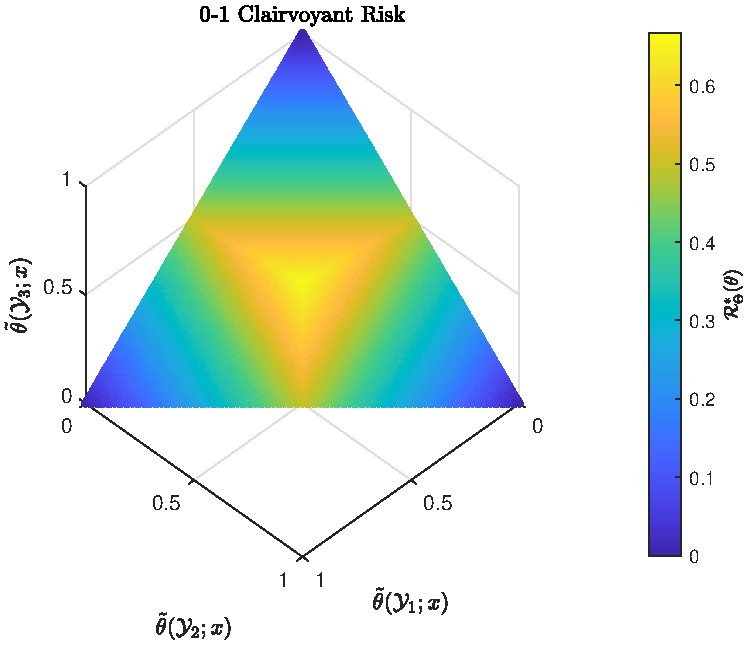
\includegraphics[width=0.9\linewidth]{Risk_clv_01_tilde.pdf}
%\caption{}
\label{fig:Risk_clv_01}
\end{figure}

\end{column}

\end{columns}
\vspace{0.75em}
\centering
\fcolorbox{bumper}{bumper}{\color{white}
\parbox{36em}{
\centering
\large
\textbf{Clairvoyant Risk $=$ Lower Bound for Conditional Risk}
}
}

\footcitetext{kay-det}


\end{frame}








\begin{frame}
\frametitle{Human Recognition Tasks}
\framesubtitle{Part I}

\begin{itemize}
\item Our recognition abilities can be partially attributed to the immeasurable volume of \alert{training data} that we consume, but we also have a type of \alert{prior knowledge}
\end{itemize}


\begin{columns}[c]

\hspace{2ex}
\begin{column}{.5\linewidth}

\begin{itemize}
\item Our sensory inputs are highly structured due to the phenomenology of the physical world
\vspace{1em}
\item Non-invertible feature extraction occurs before memorization - we possess a mechanism for ``dimensionality reduction''
\end{itemize}

\end{column}


%\vrule
%\hspace{1ex}


\begin{column}{.5\linewidth}

\begin{figure}
\centering
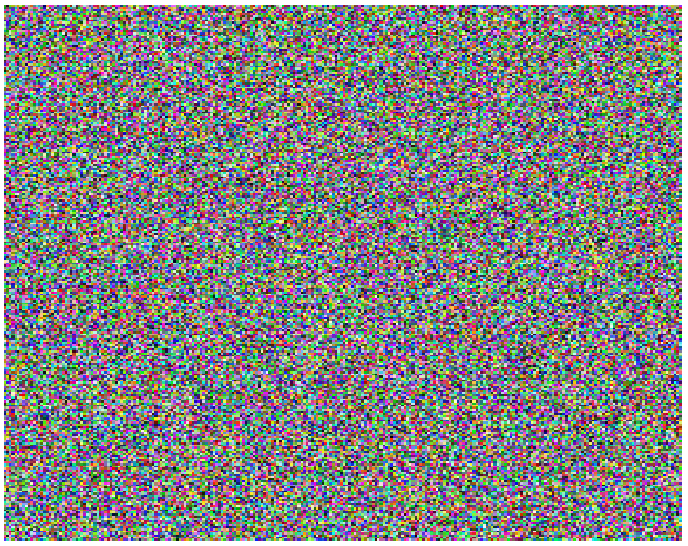
\includegraphics[width=0.7\linewidth]{RGB_random.pdf}
\caption{Randomly generated RGB image}
\label{fig:RGB_random}
\end{figure}

\end{column}

\end{columns}

\end{frame}






\begin{frame}
\frametitle{Human Recognition Tasks}
\framesubtitle{Part II}


\begin{columns}[c]

\begin{column}{.5\linewidth}

\begin{itemize}
\item \textbf{Perspective}: the labels we use are \alert{extrinsic} to our observations

\vspace{-1em}
\Large
\begin{equation*} 
\Downarrow
\end{equation*}
\normalsize

\item We defined the classes ourselves, ensuring joint probability distributions that lead to \alert{low clairvoyant risk}

\vspace{-1em}
\Large
\begin{equation*} 
\Downarrow
\end{equation*}
\normalsize

\item With accurate prior knowledge, parametric decision functions that \alert{achieve minimal risk} are possible
\end{itemize}

\end{column}


%\vrule
%\hspace{1ex}


\begin{column}{.5\linewidth}

\begin{figure}
\centering
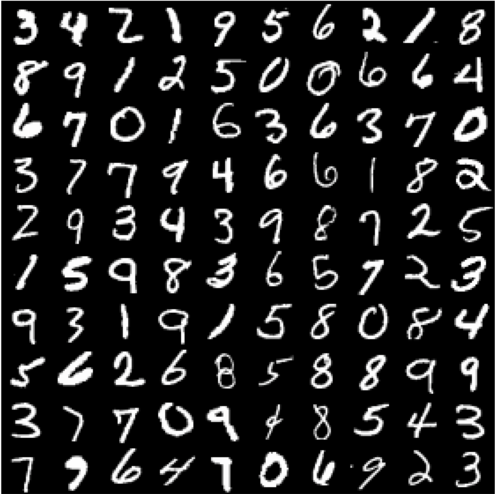
\includegraphics[width=0.7\linewidth]{mnist_digit_ex.png}
\caption{Handwritten digit samples from the MNIST Database \footnotemark}
\label{fig:mnist_digit_ex}
\end{figure}

\end{column}

\end{columns}
\vspace{0.5em}

\footcitetext{lecun-mnist}

\end{frame}








\section{Related Work}


\begin{frame}
\frametitle{Statistical Learning Work}

\begin{itemize}
\item Fundamental results in classical statistics include the existence of asymptotically consistent estimators \footfullcite{stone} and the development of error bounds for empirical risk minimization \footfullcite{vapnik}
\vspace{0.5em}
\item Practical methods for prediction in supervised Bayesian learning will be relevant for certain priors
	\vspace{0.25em}
	\begin{itemize}
	\item Approximate inference methods such as variational approximation \footfullcite{beal} enable posterior evaluation for intractable problems
	\vspace{0.25em}
	\item Non-deterministic approaches including Markov chain Monte Carlo (MCMC) methods \footfullcite{hastings} provide estimates of the predictive distribution
	\end{itemize}
\vspace{0.5em}
\item Dirichlet processes have been considered in non-parametric learning, but typically only for unsupervised learning with infinite numbers of clusters \footfullcite{gershman}
\end{itemize}
\vspace{0.5em}

\end{frame}



\begin{frame}
\frametitle{Feature Extraction for Speech/Image Recognition}

\begin{itemize}
\item Our sensory processing systems decompose information at a variety of scales - multiresolution signal decomposition with wavelet representations \footfullcite{mallat-wavtour} is popular for these learning applications
\vspace{1em}
\item For tasks such as optical character recognition (OCR), the translation dependency of a feature can significantly raise the probability of error; reconciling our desire for features that describe spatial locality with the need for translation-invariant representation is challenging
	\vspace{0.25em}
	\begin{itemize}
	\item Even popular features such as those based on multiresolution wavelet transformations \footfullcite{mallat-multires} do not provide both
	\vspace{0.25em}
	\item Focused research on shift-invariant features for 2-dimensional data \footfullcite{marco} aims to ensure this property
	\end{itemize}
\end{itemize}

\end{frame}









\section{Approach}


\begin{frame}
\frametitle{Generalized Bayesian Framework}

\begin{itemize}
\item Having motivated the perspective that \emph{all} machine learning algorithms either implicitly or explicitly use prior knowledge, this thesis will focus on a strictly \alert{Bayesian approach} to parametric supervised learning
\vspace{1em}
\item Existing treatments of parametric Bayesian learning effect \underline{significant} data dimensionality reduction and yet fail to sufficiently consider the implications of how the mapping between the parameters and the probability model is selected
\vspace{1em}
\item Designs using both \alert{full support} and \alert{limited support} prior distributions will be analyzed and subsequently applied to human recognition tasks
\end{itemize}

\end{frame}


\begin{frame}
\frametitle{Bayesian Inference}


\large
\begin{equation*} 
\Downarrow \quad \Downarrow \quad \textbf{\textit{Model Unknown. Select Prior }} \bm{\mathrm{p}_\uptheta} \quad \Downarrow \quad \Downarrow 
\end{equation*}
\normalsize
\begin{IEEEeqnarray*}{rCl} \label{eq:risk}
\Rcal(f) & = & \Erm_{\uptheta}\big[ \Rcal_{\Theta}(f ; \uptheta) \big] = \Erm_{\Drm}\Bigg[ \Erm_{\xrm | \Drm}\bigg[ \Erm_{\yrm | \xrm,\Drm} \Big[ \Lcal\big( f(\xrm;\Drm),\yrm \big) \Big] \bigg] \Bigg]
\end{IEEEeqnarray*}

\vspace{-0.5em}
\hrulefill
\vspace{0.5em}

\begin{columns}[c]

\begin{column}{.5\linewidth}

\textbf{Optimal Decision}: 
\begin{IEEEeqnarray}{rCl} \label{eq:f_opt_xD}
f^*(\xrm;\Drm) & = & \argmin_{h \in \Hcal} \Erm_{\yrm | \xrm,\Drm}\big[ \Lcal(h,\yrm) \big] \nonumber
\end{IEEEeqnarray}

\textbf{Minimum Bayes Risk}:
\begin{IEEEeqnarray}{rCl} \label{eq:risk_min}
\Rcal^* & \equiv & \Erm_{\Drm} \Bigg[ \Erm_{\xrm | \Drm} \bigg[ \min_{h \in \Hcal} \Erm_{\yrm | \xrm,\Drm}\big[ \Lcal(h,\yrm) \big] \bigg] \Bigg] \nonumber
\end{IEEEeqnarray}

\end{column}

\begin{column}{.5\linewidth}

\begin{block}{Predictive Distributions}

Bayesian PMF is the conditional expectation of the true PMF $\Prm_{\yrm | \xrm,\uptheta} \equiv \tilde{\uptheta}(\xrm)$:
\large
\begin{equation*}
\Prm_{\yrm | \xrm,\Drm} = \Erm_{\uptheta | \xrm,\Drm}\big[ \Prm_{\yrm | \xrm,\uptheta} \big] \equiv \mu_{\tilde{\uptheta}(\xrm) | \xrm,\Drm}
\end{equation*}


\end{block}

\end{column}

\end{columns}


\end{frame}





\begin{frame}
\frametitle{Training Data Sufficient Statistic}

\begin{columns}[c]


\begin{column}{.5\linewidth}

\textbf{Likelihood Function}:
\begin{IEEEeqnarray}{C}
\Prm_{\Drm | \uptheta}(D | \theta) = \prod_{y \in \Ycal} \prod_{x \in \Xcal} \theta(y,x)^{\bar{N}(y,x;D)} \nonumber 
\end{IEEEeqnarray}

\textit{Transform}: $\bar{N} : \Dcal \mapsto \bar{\Ncal}$
\vspace{0.25em}
$\bar{N}(y,x;D) = \sum_{n=1}^N \delta\big[ (y,x),D_n \big]$
 
\begin{equation*}
\bar{\Ncal} = \left\{ \bar{n} \in {\Zbb_{\geq 0}}^{\Ycal \times \Xcal}: \sum_{y \in \Ycal} \sum_{x \in \Xcal} \bar{n}(y,x) = N \right\}
\end{equation*}

\end{column}

\vrule
\hspace{0.5ex}
\begin{column}{.5\linewidth}

\begin{itemize}
\item Empirical count $\bar{N}(\Drm)$ is a \alert{sufficient statistic}\footnotemark ~for the model $\uptheta$
\vspace{0.5em}
\item $|\bar{\Ncal}| = \binom{N+|\Ycal||\Xcal|-1}{|\Ycal||\Xcal|-1} \leq |\Dcal|$  
\vspace{0.5em}
%\begin{itemize}
%\item [$\Rightarrow$] \large \textbf{Efficient Transform} \normalsize
%\end{itemize}
\end{itemize}

\vspace{-1.5em}
 
\Large
\begin{equation*} 
\Downarrow \quad \Downarrow
\end{equation*}
\normalsize
\vspace{-1.5em}
\begin{block}{Efficient Representation}
\centering
\textbf{Express distributions using new \\random process $\nbarrm \equiv \bar{N}(\Drm) \in \bar{\Ncal}$}
\end{block}

\vspace{1em}
\begin{itemize}
\item[$*$] ``Marginal'' process: $\nrm' \equiv \sum_{y \in \Ycal} \nbarrm(y,\cdot)$ 
\end{itemize}


\end{column}

\end{columns}

\footcitetext{bernardo}

\end{frame}





\begin{frame}
\frametitle{Full Support Priors}

\begin{itemize}
\item Full support priors are necessary to ensure \alert{asymptotically consistent} estimation of any model $\theta$ and thus optimal decisions in the limit of training data volume $N$
\vspace{0.5em}
\item Often, priors are termed non-informative as long as they are approximately uniform over their limited support - to be \emph{truly} non-informative, the prior must have full support
\vspace{0.5em}
\item The \alert{Dirichlet distribution} has full support over the space of data-generating distributions and can be parameterized in different ways to achieve both informative and non-informative priors
	\vspace{0.25em}
	\begin{itemize}
	\item Additionally, it is a \emph{conjugate prior} for likelihood functions in the exponential family \footfullcite{theodoridis-ML}, enabling tractable posterior evaluation for I.I.D. training data
	\end{itemize}
\end{itemize}

\end{frame}





\begin{frame}
\frametitle{Dirichlet Prior Distribution}
\framesubtitle{Part I}

\begin{itemize}
\item The model probability density function (PDF) is Dirichlet \footfullcite{bishop} with parameters $\alpha : \Ycal \times \Xcal \mapsto \Rbb^+$:
\end{itemize}

\vspace{0.5em}
\begin{columns}[c]

\begin{column}{.45\linewidth}

\textbf{\underline{Joint Model}}:
\vspace{-0.25em}
\begin{IEEEeqnarray*}{rCl}
\prm_{\uptheta}(\theta) & = & \Dir\big( \theta ; \alpha \big) \\
& = & \beta(\alpha)^{-1} \prod_{y \in \Ycal} \prod_{x \in \Xcal} \theta(y,x)^{\alpha(y,x) - 1} \\
\end{IEEEeqnarray*}

\small
\textit{Concentration}: 
$\alpha_0 \equiv \sum_{y \in \Ycal} \sum_{x \in \Xcal} \alpha(y,x)$
\normalsize

\end{column}

%\hspace{1ex}
\huge
\begin{column}{.1\linewidth}
$\Rightarrow$ \\ $\Rightarrow$ 
\end{column}
\normalsize
\hspace{-5ex}

\begin{column}{.45\linewidth}

\textbf{\underline{Conditional Model}}:
\vspace{-0.25em}
\begin{IEEEeqnarray*}{rCl}
\prm_{\tilde{\uptheta} | \uptheta'}\big( \tilde{\theta} | \theta' \big) & = & \prm_{\tilde{\uptheta}}\big( \tilde{\theta} \big) \\
& = & \prod_{x \in \Xcal} \Dir\Big( \tilde{\theta}(x) ; \alpha(\cdot,x) \Big) \\
\end{IEEEeqnarray*}

\small
\textit{Concentration}: 
$\alpha'(x) \equiv \sum_{y \in \Ycal} \alpha(y,x)$
\normalsize

\end{column}

\end{columns}


\vspace{1em}
\centering
\fcolorbox{bumper}{bumper}{\color{white}
\parbox{36em}{
\centering
\large
\textbf{True predictive distribution $\bm{\tilde{\uptheta}}$ is independent of the marginal \\model $\bm{\uptheta'}$ and inherits a Dirichlet PDF}
}
}

\end{frame}



\begin{frame}
\frametitle{Dirichlet Prior Distribution}
\framesubtitle{Part II: Concentration Trends}

\begin{itemize}
\item Non-informative: $\alpha = 1$ creates the uniform Dirichlet prior, $\prm_{\uptheta} = \big( |\Ycal||\Xcal|-1 \big)!$
\vspace{0.5em}
\item Maximal ($\alpha_0 \to \infty$) and minimal ($\alpha_0 \to 0$) localization around mean $\mu_{\uptheta} = \frac{\alpha}{\alpha_0}$
\end{itemize}

\begin{figure}
\centering
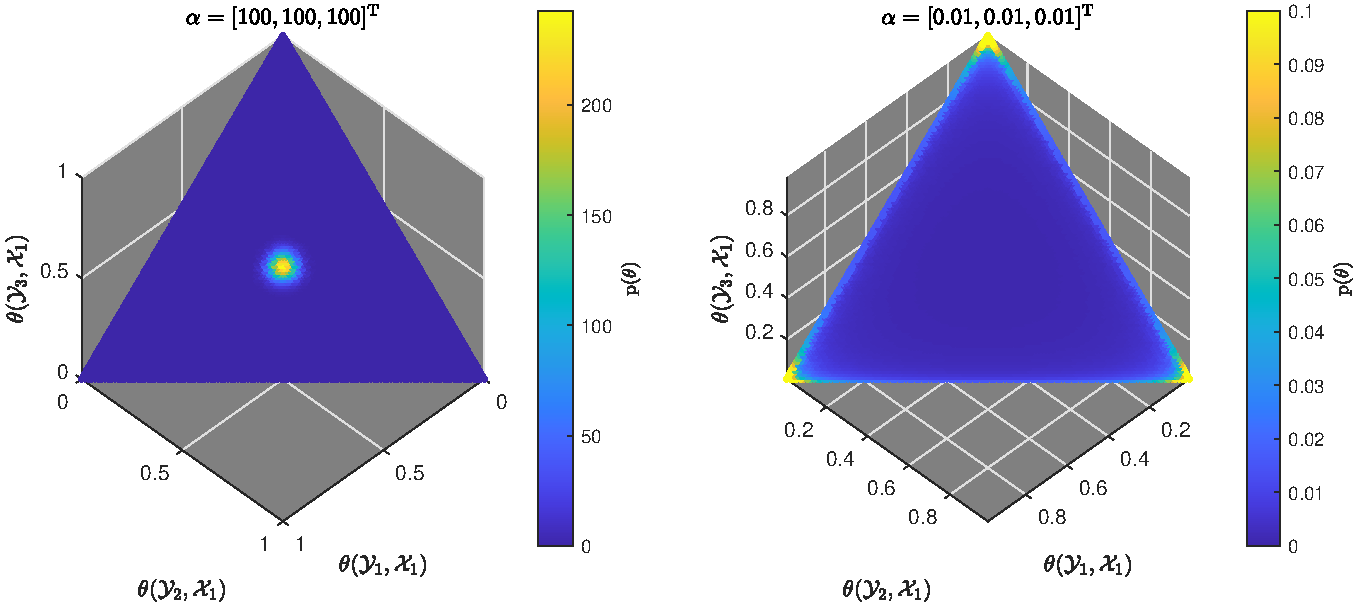
\includegraphics[width=0.8\linewidth]{P_theta_hrz.pdf}
%\caption{Minimum 0--1 Risk for different numbers of possible observations}
%\label{fig:Risk_01_uni_N_leg_Mx}
\end{figure}


\end{frame}




\begin{frame}
\frametitle{Limited Support Priors}

\begin{itemize}
\item The most informative priors have limited support, specifically, support of \alert{limited dimensionality}, such that $\dim(\Theta) < |\Ycal||\Xcal| - 1$
\vspace{0.5em}
\item The performance trade-offs dependent on the support dimensionality will be a primary focus
	\vspace{0.25em}
	\begin{itemize}
	\item Potential risk reduction relative to full support priors for data-limited problems
	\vspace{0.25em}
	\item Failure to meet the clairvoyant risk in the limit of increasing training data volume
	\end{itemize}
%\vspace{0.5em}
%\item asd
\vspace{0.5em}
\item Special attention will be given to the design of low-dimensionality support sets that are sensible for human recognition tasks
\end{itemize}

\vspace{1em}
\centering
\fcolorbox{bumper}{bumper}{\color{white}
\parbox{36em}{
\centering
\large
\textbf{Fewer degrees of freedom needed to characterize the support \\ $\Downarrow$ \\Minimal risk achievable by simpler parametric functions}
}
}

\end{frame}



\begin{frame}
\frametitle{Informative Priors for Human Recognition Tasks}
\framesubtitle{Part I: Data Dimensionality}



\begin{columns}[c]

\begin{column}{.5\linewidth}

\begin{itemize}
\item Data processed during human recognition is highly structured

\vspace{-1em}
\Large
\begin{equation*}
\Downarrow
\end{equation*}
\normalsize

\item Relatively low \emph{intrinsic dimensionality}, limited support data model $\theta'$

\vspace{-1em}
\Large
\begin{equation*}
\Downarrow
\end{equation*}
\normalsize
\end{itemize}

\vspace{-1.5em}
\begin{IEEEeqnarray*}{rCl}
\big\| \theta' \big\|_0 & = & \sum_{x \in \Xcal} \Big(1 - \delta[\theta'(x),0] \Big) \leq M_{\Xcal} < |\Xcal| 
\end{IEEEeqnarray*}

%\vspace{1em}
%\centering
%
%\textbf{Fewer degrees of freedom needed to characterize the support}
%
%\vspace{-2em}
%\Large
%\begin{equation*} 
%\Downarrow
%\end{equation*}
%\normalsize
%
%\textbf{Minimal risk can be achieved with \alert{simpler} parametric functions}

\end{column}

\begin{column}{.5\linewidth}

\begin{figure}
\centering
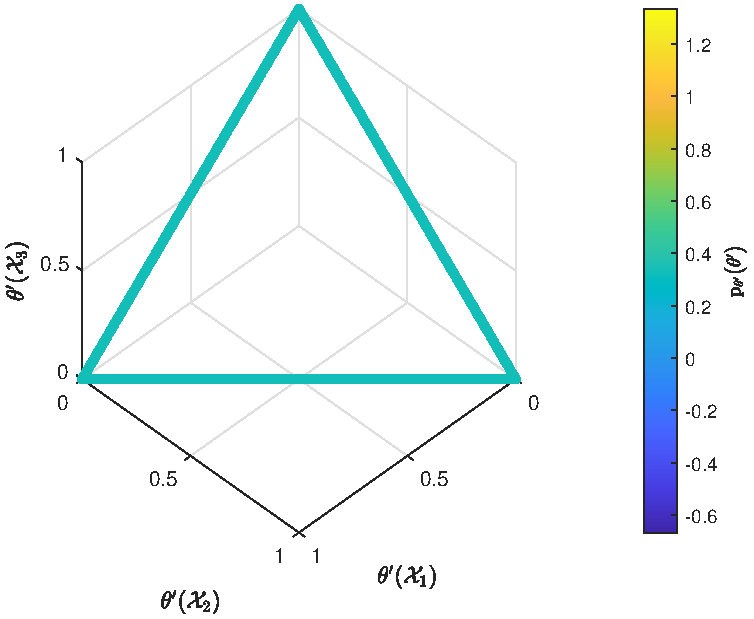
\includegraphics[width=0.9\linewidth]{P_theta_limited_obs.pdf}
\caption{Marginal model prior for $\big\| \theta' \big\|_0 \leq 2$}
\label{fig:P_theta_limited_obs}
\end{figure}

\end{column}

\end{columns}

\end{frame}




\begin{frame}
\frametitle{Informative Priors for Human Recognition Tasks}
\framesubtitle{Part II: Sufficient Statistics}

\begin{itemize}
\item Our internal ``pre-processing'' greatly reduces the complexity of our sensory input

\vspace{-1em}
\Large
\begin{equation*} 
\Downarrow
\end{equation*}
\normalsize

\item Parametric learning functions should be able to perform feature extraction and effect significant dimensionality reduction \alert{without any loss of performance}

\vspace{-1em}
\Large
\begin{equation*} 
\Downarrow
\end{equation*}
\normalsize

\item The prior distribution's support should be limited to a subspace that guarantees a low-dimensional \alert{sufficient statistic}
\end{itemize}


\end{frame}




\begin{frame}
\frametitle{Informative Priors for Human Recognition Tasks}
\framesubtitle{Part II: Sufficient Statistics}


\begin{columns}[T]

\begin{column}{.5\linewidth}

\begin{itemize}
\item Define transform $T: \Xcal \mapsto \Tcal$, such that $\Xcal_{\srm}(t) = \big\{ x \in \Xcal : T(x) = t \big\}$
\vspace{0.5em}
\item \textbf{Data reduction}: $|\Tcal| < |\Xcal|$
\end{itemize}

\vspace{1.5em}
\begin{block}{Sufficiency}
Statistic $\trm \equiv T(\xrm)$ must satisfy\footnotemark
\begin{IEEEeqnarray*}{rCl}
\Prm_{\xrm | \uptheta',\trm}(x | \theta',t) & = & \frac{\theta'(x)}{\sum_{x' \in \Xcal_{\srm}(t)} \theta'(x')} = g(x;t)
\end{IEEEeqnarray*}
$\forall  \: x \in \Xcal_s(t), \; t \in \Tcal$, with no additional dependency on the model
\end{block}



\end{column}

\begin{column}{.5\linewidth}

\begin{figure}
\centering
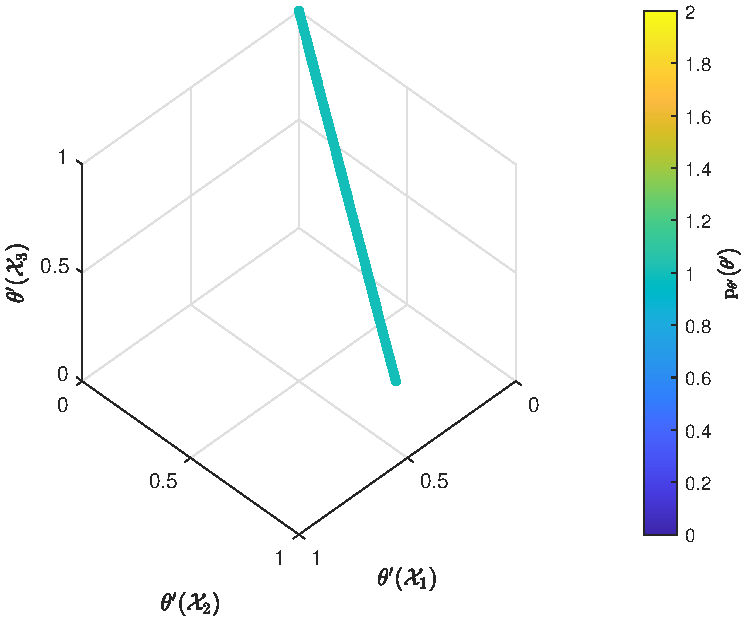
\includegraphics[width=0.9\linewidth]{P_theta_suff_stat.pdf}
\caption{A marginal model prior for $|\Tcal| = 2$}
\label{fig:P_theta_suff_stat}
\end{figure}

\end{column}

\end{columns}
\vspace{0.5em}

\footcitetext{kay-est}

\end{frame}



\begin{frame}
\frametitle{Informative Priors for Human Recognition Tasks}
\framesubtitle{Part III: Low Risk Prediction}

\begin{columns}[c]

\begin{column}{.6\linewidth}

\begin{itemize}
\item Humans effectively perform \emph{unsupervised learning} on sensory observations, creating a joint distribution $\theta$ that leads to low clairvoyant risk $\Rcal_{\Theta}^*(\theta)$

\vspace{-1em}
\Large
\begin{equation*} 
\Downarrow \quad \Downarrow
\end{equation*}
\normalsize

\vspace{0.5em}
\item The true predictive models $\tilde{\theta}(x)$ should be highly definitive, having \alert{low entropy} or demonstrating \alert{sparsity}

\end{itemize}



\end{column}

\begin{column}{.4\linewidth}

\begin{figure}
\centering
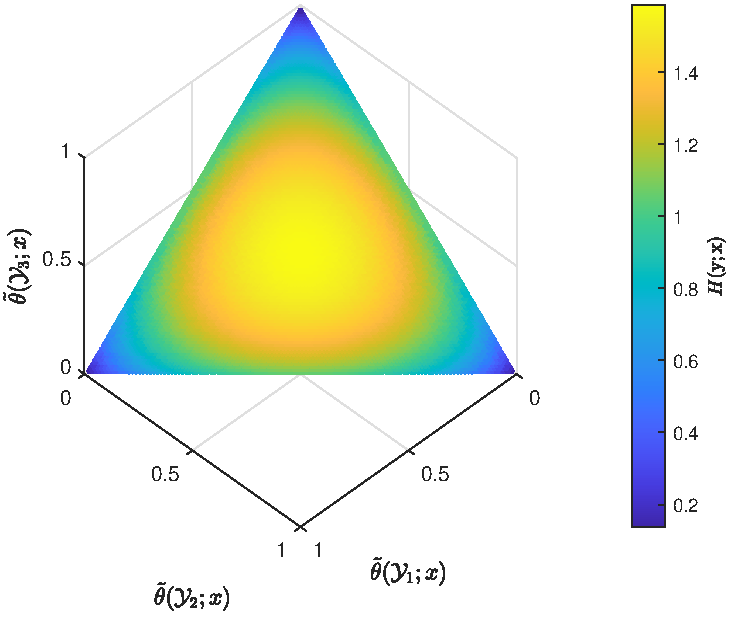
\includegraphics[width=1\linewidth]{theta_tilde_entropy.pdf}
\caption{Conditional entropy for $\tilde{\theta}(x)$}
\label{fig:theta_tilde_entropy}
\end{figure}

\end{column}

\end{columns}

\end{frame}




\begin{frame}
\frametitle{Informative Priors for Human Recognition Tasks}
\framesubtitle{Part III: Low Risk Prediction}




\begin{columns}[c]

\begin{column}{.3\linewidth}

\textbf{$L^p$-norm restrictions}:
%
\vspace{0.5em}
\begin{IEEEeqnarray*}{rCl}
\big\| \tilde{\theta}(x) \big\|_{\infty} & = & \max_{y \in \Ycal} \big| \tilde{\theta}(y;x) \big| \\
& \geq & \rho > 1/|\Ycal|
\end{IEEEeqnarray*}
%
\begin{equation*}
\big\| \tilde{\theta}(x) \big\|_0 \leq M_{\Ycal} < |\Ycal|
\end{equation*}

\end{column}

\begin{column}{.35\linewidth}

\begin{figure}
\centering
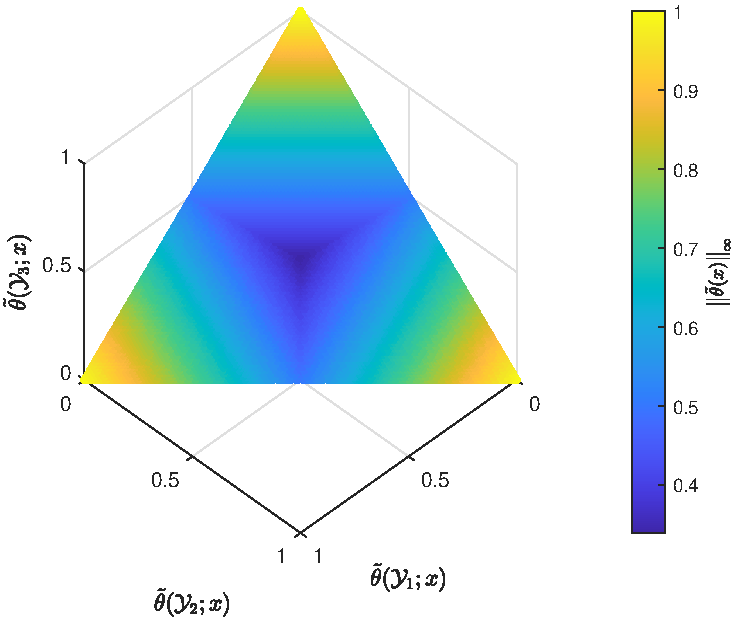
\includegraphics[width=1\linewidth]{theta_tilde_Linf.pdf}
%\caption{$L^{\infty}$-norm of $\tilde{\theta}(x)$}
%\label{fig:theta_tilde_Linf}
\end{figure}


\end{column}

\begin{column}{.35\linewidth}

\begin{figure}
\centering
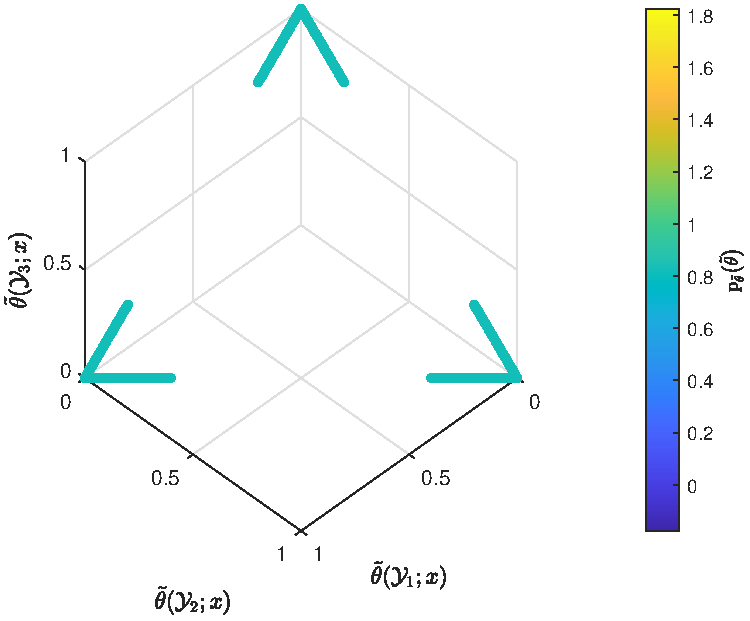
\includegraphics[width=1\linewidth]{theta_tilde_L0-inf.pdf}
%\caption{Limited support for $\tilde{\theta}(x)$, $\big\| \tilde{\theta}(x) \big\|_0 \leq 2$, $\big\| \tilde{\theta}(x) \big\|_{\infty} \geq 0.8$}
%\label{fig:theta_tilde_L0-inf}
\end{figure}

\end{column}

\end{columns}


\vspace{1.5em}
\centering
\fcolorbox{bumper}{bumper}{\color{white}
\parbox{36em}{
\centering
\large
\textbf{Condition $\bm{\big\| \tilde{\theta}(x) \big\|_{\infty} = 1}$ restricts the support of the predictive model to a countable set, limiting computational complexity of implementation}
}
}

\end{frame}






\section{Preliminary Results}


\begin{frame} 
\frametitle{Publications}

\begin{itemize}
\item Initial work has focused on optimal decision functions derived from Dirichlet prior distributions for finite sets $\Ycal$ and $\Xcal$
\vspace{0.5em}
\item Risk analysis of resultant Bayesian estimates and hypotheses for regression and classification, respectively, has been performed
\vspace{0.5em}
\item \alert{Publications to date}:
	\vspace{0.25em}
	\begin{itemize}
	\item \emph{Predictive Distribution Estimation for Bayesian Machine Learning using a Dirichlet Prior}, presented at 	the 53rd Annual Asilomar Conference on Signals, Systems, and Computers
	\vspace{0.25em}
	\item \emph{Bayesian Learning for Classification using a Uniform Dirichlet Prior}, presented at the 7th IEEE Global Conference on Signal and Information Processing
	\end{itemize}
\end{itemize}

\end{frame}



\begin{frame} 
\frametitle{Training Data Characterization}


\begin{columns}[T]

\begin{column}{.45\linewidth}

\textbf{Empirical Statistic Likelihood}:
\begin{IEEEeqnarray*}{rCl}
\Prm_{\nbarrm | \uptheta}(\bar{n} | \theta) & = & \Multi(\bar{n}; N,\theta) \\
& = & \Mcal(\bar{n}) \prod_{y \in \Ycal} \prod_{x \in \Xcal} \theta(y,x)^{\bar{n}(y,x)} 
\end{IEEEeqnarray*}

\small
\vspace{1em}
\textit{Marginal Statistic}: $\nrm' | \uptheta \sim \Multi(N,\uptheta')$

\vspace{1em}
\textit{Conditional Statistic}: $\nbarrm(\cdot,x) | \nrm'(x),\uptheta \sim \Multi\big( \nrm'(x),\tilde{\uptheta}(x) \big)$
\normalsize

\end{column}

\hspace{2ex}
\huge
\begin{column}{.1\linewidth}
\vspace{2em}
$\Rightarrow$ 

\vspace{2em}

$\Rightarrow$ 
\end{column}
\normalsize
\hspace{-3ex}

\begin{column}{.45\linewidth}

\textbf{Statistic ``Evidence''}:
\begin{IEEEeqnarray*}{rCl}
\Prm_{\nbarrm}(\bar{n}) & = & \DM(\bar{n}; N,\alpha) \\
& = & \Mcal(\bar{n}) \beta(\alpha)^{-1} \beta(\alpha + \bar{n})
\end{IEEEeqnarray*}

\small
\vspace{2em}
\textit{Marginal Statistic}: 

$\nrm' \sim \DM(N,\alpha')$

\vspace{1em}
\textit{Conditional Statistic}: $\nbarrm(\cdot,x) | \nrm'(x) \sim \DM\big( \nrm'(x),\alpha(\cdot,x) \big)$
\normalsize

\end{column}

\end{columns}



\vspace{1em}
\centering
\fcolorbox{bumper}{bumper}{\color{white}
\parbox{36em}{
\centering
\large
\textbf{Dirichlet Prior leads to tractable Dirichlet-Multinomial\footfullcite{johnson} Evidence function}
}
}

\vspace{0.5em}


\end{frame}





\begin{frame}
\frametitle{Model Posterior Distribution}
\framesubtitle{Part I: Closed-Form}

\begin{itemize}
\item Independence of $\tilde{\uptheta}$ from $\uptheta'$ implies conditional independence of $\tilde{\uptheta}$ from $\xrm$ given $\nbarrm$
	\vspace{0.25em}
	\begin{itemize}
	\item No ``unsupervised'' inference is possible 
	\end{itemize}
\vspace{0.5em}
\item Since the likelihood $\Prm_{\nbarrm | \uptheta}$ has exponential form, the Dirichlet PDF is a conjugate prior 
\end{itemize}
\vspace{0.25em}
\begin{IEEEeqnarray*}{rCl}
\prm_{\tilde{\uptheta} | \nbarrm,\xrm}\big( \tilde{\theta} | \bar{n},x \big) = \prm_{\tilde{\uptheta} | \nbarrm}\big( \tilde{\theta} | \bar{n} \big) & = & \prod_{x' \in \Xcal} \prm_{\tilde{\uptheta}(x') | \nbarrm(\cdot,x')}\big(\tilde{\theta}(x') | \bar{n}(\cdot,x') \big) \\
& = & \prod_{x' \in \Xcal} \Dir\big( \tilde{\theta}(x') ; \alpha(\cdot,x') + \bar{n}(\cdot,x') \big) \nonumber
\end{IEEEeqnarray*}

\vspace{0.5em}

\centering
\fcolorbox{bumper}{bumper}{\color{white}
\parbox{36em}{
\centering
\large
\textbf{Posterior for model $\bm{\tilde{\uptheta}(x)}$ is Dirichlet and dependent \\solely on the sufficient statistic elements $\bm{\nbarrm(\cdot,x)}$}
}
}

\end{frame}



\begin{frame}
\frametitle{Model Posterior Distribution}
\framesubtitle{Part II: Asymptotic Trends}

\begin{columns}[T]

\begin{column}{.55\linewidth}

\begin{itemize}
\item Covariance of Dirichlet $\prm_{\tilde{\uptheta}(x) | \nbarrm(\cdot,x)}$ decreases monotonically with concentration $\alpha'(x)+n'(x)$
%\item Localized around $\mu_{\tilde{\uptheta}(x) | \nbarrm(\cdot,x)}$
\end{itemize}
\Large
\begin{equation*} 
\Downarrow \quad \Downarrow
\end{equation*}
\normalsize
\begin{itemize}
\vspace{-1em}
\item As $n'(x) \to \infty$, the posteriors tend to 
\begin{IEEEeqnarray*}{L}
\prm_{\tilde{\uptheta}(x) | \nbarrm(\cdot,x)}\Big(\tilde{\theta}(x) | \bar{n}(\cdot,x) \Big) \to \delta\left( \tilde{\theta}(x) - \mu_{\tilde{\uptheta}(x) | \nbarrm(\cdot,x)} \right)
\end{IEEEeqnarray*}
\end{itemize}

\vspace{1em}

\centering
\fcolorbox{bumper}{bumper}{\color{white}
\parbox{22em}{
\centering
\large
\textbf{Asymptotically consistent estimation of $\bm{\tilde{\uptheta}}$ due to full support of prior}
}
}

\end{column}

\hspace{3ex}
\begin{column}{.45\linewidth}
\vspace{-1.5em}
\begin{figure}
\centering
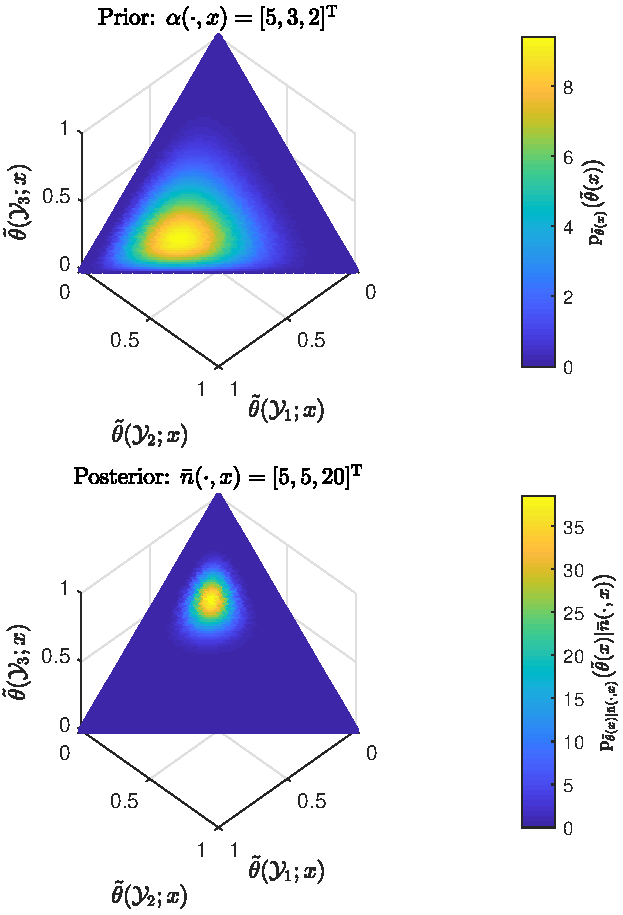
\includegraphics[width=0.8\linewidth]{P_theta_post_tilde.pdf}
%\caption{}
\end{figure}

\end{column}

\end{columns}

\end{frame}




\begin{frame}
\frametitle{Bayesian Predictive Distribution}

\textit{The Bayesian predictive distribution is a convex combination of two conditional PMF's}:
\vspace{0.5em}
\begin{IEEEeqnarray*}{rCl} \label{P_y_xD_uniform}
\Prm_{\yrm | \xrm,\nbarrm}(\cdot | x,\bar{n}) & = & \mu_{\tilde{\uptheta}(x) | \nbarrm(\cdot,x)}\big( \bar{n}(\cdot,x) \big) \\
& \equiv & \left(\frac{\alpha'(x)}{\alpha'(x) + n'(x)}\right) \frac{\alpha(\cdot,x)}{\alpha'(x)} + \left(\frac{n'(x)}{\alpha'(x) + n'(x)}\right) \frac{\bar{n}(\cdot,x)}{n'(x)}
\end{IEEEeqnarray*}

\vspace{0.5em}

\begin{description}
\item[Prior Mean] Uniform PMF $\mu_{\tilde{\uptheta}(x)} = \alpha(\cdot,x) / \alpha'(x)$ dependent only on the Dirichlet parameterization
\vspace{0.25em}
\item[Conditional Empirical PMF] $\bar{n}(\cdot,x) / n'(x)$ dependent only on training data
\end{description}

\vspace{1em}

\centering
\fcolorbox{bumper}{bumper}{\color{white}
\parbox{36em}{
\centering
\large
\textbf{As the data volume $\bm{n'(x)}$ increases relative to the concentration $\bm{\alpha'(x)}$, the predictive distribution tends toward the empirical PMF}
}
}

\end{frame}



\begin{frame}
\frametitle{Model Estimation Perspective}
\framesubtitle{Part I}

\textbf{Assess estimation of $\theta$ using a difference process}: $\Delta(\xrm,\nbarrm,\uptheta) \equiv \Prm_{\yrm | \xrm,\nbarrm} - \Prm_{\yrm | \xrm,\uptheta}$

\begin{columns}[c]

\begin{column}{.7\linewidth}

\vspace{-1.5em}
\small
\begin{IEEEeqnarray*}{rCl} \label{eq:predictive_bias}
\mathrm{Bias}(\xrm,\nrm',\uptheta) & = & \Erm_{\nbarrm | \nrm',\uptheta}\big[ \Delta(\xrm,\nbarrm,\uptheta) \big] \\
& = & \frac{\alpha'(\xrm)}{\alpha'(\xrm) + \nrm'(\xrm)} \left( \frac{\alpha(\cdot,\xrm)}{\alpha'(\xrm)} - \tilde{\uptheta}(\xrm) \right) 
\end{IEEEeqnarray*}
\vspace{0em}
\begin{IEEEeqnarray*}{L} \label{eq:predictive_cov}
\mathrm{Cov}(y,y';\xrm,\nrm',\uptheta) = \Crm_{\nbarrm | \nrm',\uptheta} \big[\Prm_{\yrm | \xrm,\nbarrm}(\cdot | \xrm,\nbarrm) \big](y,y') \\
\qquad = \frac{\nrm'(\xrm)}{\big( \alpha'(\xrm) + \nrm'(\xrm) \big)^2} \left( \tilde{\uptheta}(y;\xrm) \delta[y,y'] - \tilde{\uptheta}(y;\xrm) \tilde{\uptheta}(y';\xrm) \right) 
\end{IEEEeqnarray*}
\normalsize

%\vspace{-1.5em}

%\Large
%\begin{equation*} 
%\Downarrow \quad \Downarrow
%\end{equation*}
%\normalsize
%
%\vspace{-2em}

%\begin{IEEEeqnarray*}{rCl} \label{eq:predictive_del_sq}
%\mathcal{E}(y,y' ; \xrm,\nrm',\uptheta) & = & \Erm_{\nbarrm | \nrm',\uptheta} \Big[ \Delta(y;\xrm,\nbarrm,\uptheta) \Delta(y';\xrm,\nbarrm,\uptheta) \Big] \\
%& = & \bm{\mathrm{Bias}(y;\xrm,\nrm',\uptheta) \mathrm{Bias}(y';\xrm,\nrm',\uptheta) + \mathrm{Cov}(y,y';\xrm,\nrm',\uptheta)}
%\end{IEEEeqnarray*}

\end{column}

\begin{column}{.3\linewidth}

\begin{table}
\renewcommand{\arraystretch}{1.5}
\begin{tabular}{| c | c |}
\hline 
$\alpha'(x)$ & Bias \\
\hhline{|=|=|}
$\to \infty$ & $\frac{\alpha(\cdot,\xrm)}{\alpha'(\xrm)} - \tilde{\uptheta}(\xrm)$ \\ 
\hline
$\to 0$ & 0 \\
\hline
\end{tabular}
%\caption{}
\end{table}

\vspace{-1em}
\begin{table}
\renewcommand{\arraystretch}{1.5}
\begin{tabular}{| c | c | }
\hline 
$\alpha'(x)$ & Covariance \\
\hhline{|=|=|}
$\to \infty$ & 0 \\ 
\hline
$\to 0$ & $\frac{\Sigma_{\nbarrm(\cdot,\xrm) | \nrm'(\xrm),\tilde{\uptheta}(\xrm)}(y,y')}{\nrm'(\xrm)^2}$ \\
\hline
\end{tabular}
%\caption{}
\end{table}

\end{column}

\end{columns}

%\small
%\begin{IEEEeqnarray*}{rCl} \label{eq:predictive_del_sq}
%\Erm_{\nbarrm | \nrm',\uptheta} \Big[ \Delta(y;\xrm,\nbarrm,\uptheta) \Delta(y';\xrm,\nbarrm,\uptheta) \Big] 
%& = & \bm{\mathrm{Bias}(y;\xrm,\nrm',\uptheta) \mathrm{Bias}(y';\xrm,\nrm',\uptheta) + \mathrm{Cov}(y,y';\xrm,\nrm',\uptheta)}
%\end{IEEEeqnarray*}

\centering
\fcolorbox{bumper}{white}{\color{black}
\parbox{36em}{
\centering
\small
$\Erm_{\nbarrm | \nrm',\uptheta} \Big[ \Delta(y;\xrm,\nbarrm,\uptheta) \Delta(y';\xrm,\nbarrm,\uptheta) \Big] 
= \mathrm{Bias}(y;\xrm,\nrm',\uptheta) \mathrm{Bias}(y';\xrm,\nrm',\uptheta) + \mathrm{Cov}(y,y';\xrm,\nrm',\uptheta)$
}
}


\end{frame}




\begin{frame}
\frametitle{Model Estimation Perspective}
\framesubtitle{Part II}

\begin{columns}[c]

\begin{column}{0.3\linewidth}

\textbf{Concentration parameter controls a Bias-Variance trade-off}

\vspace{1em}
\begin{figure}
\centering
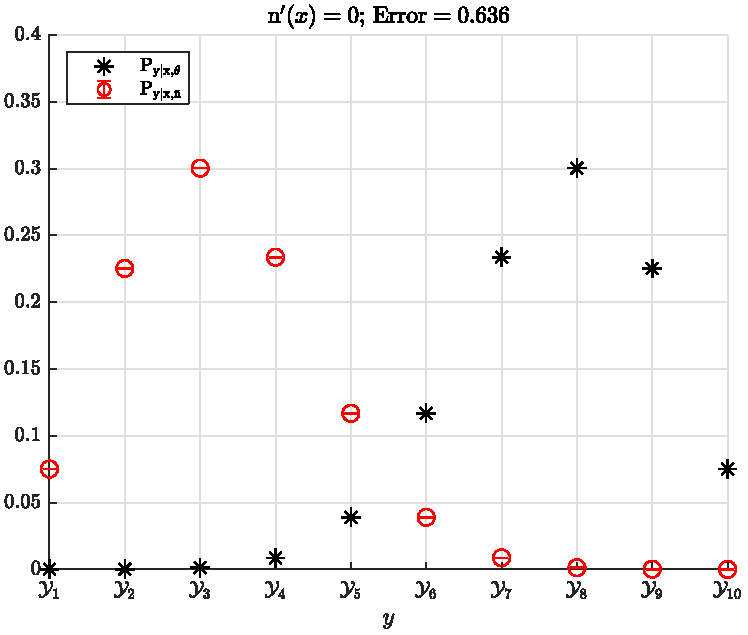
\includegraphics[width=1\linewidth]{P_yx_error_N_0.pdf}
%\caption{Model $\uptheta$ estimate, no training data}
%\label{fig:P_yx_error_N_0}
\end{figure}


\end{column}

\begin{column}{0.35\linewidth}
\begin{figure}
\centering
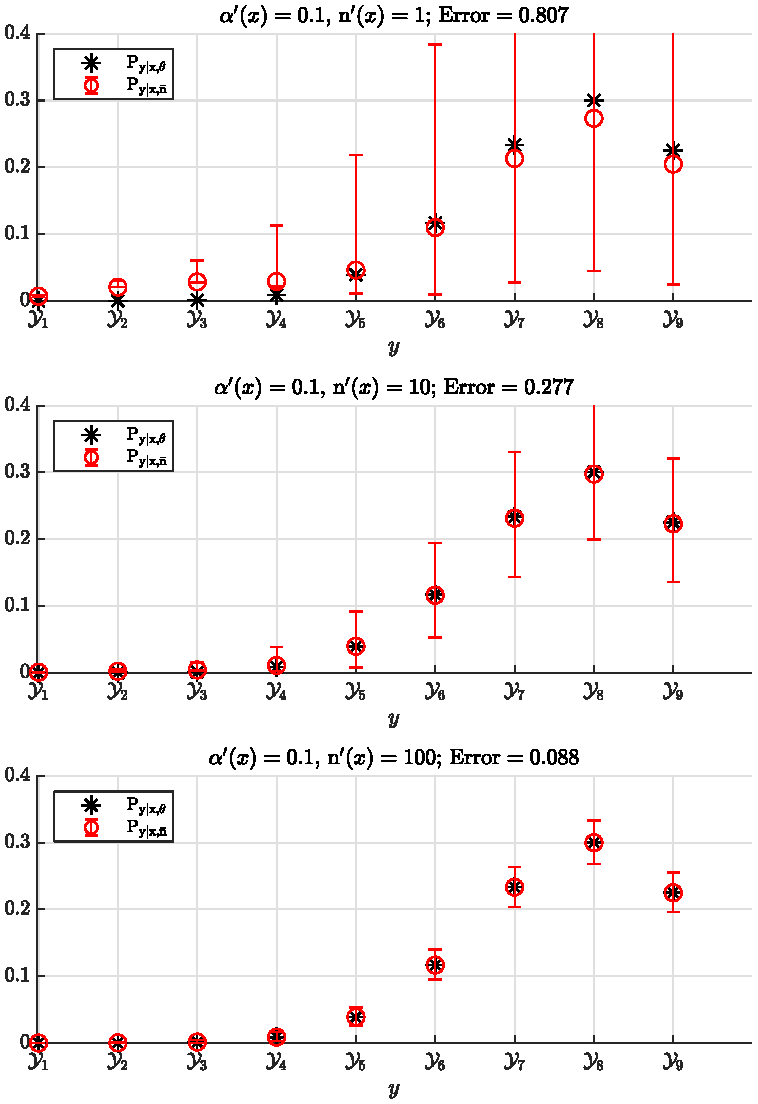
\includegraphics[width=1\linewidth]{P_yx_error_a0_0_1.pdf}
%\caption{Model $\uptheta$ estimates, $\alpha_0 = 0.1$}
%\label{fig:P_yx_error_a0_0_1}
\end{figure}
\end{column}

\begin{column}{0.35\linewidth}
\begin{figure}
\centering
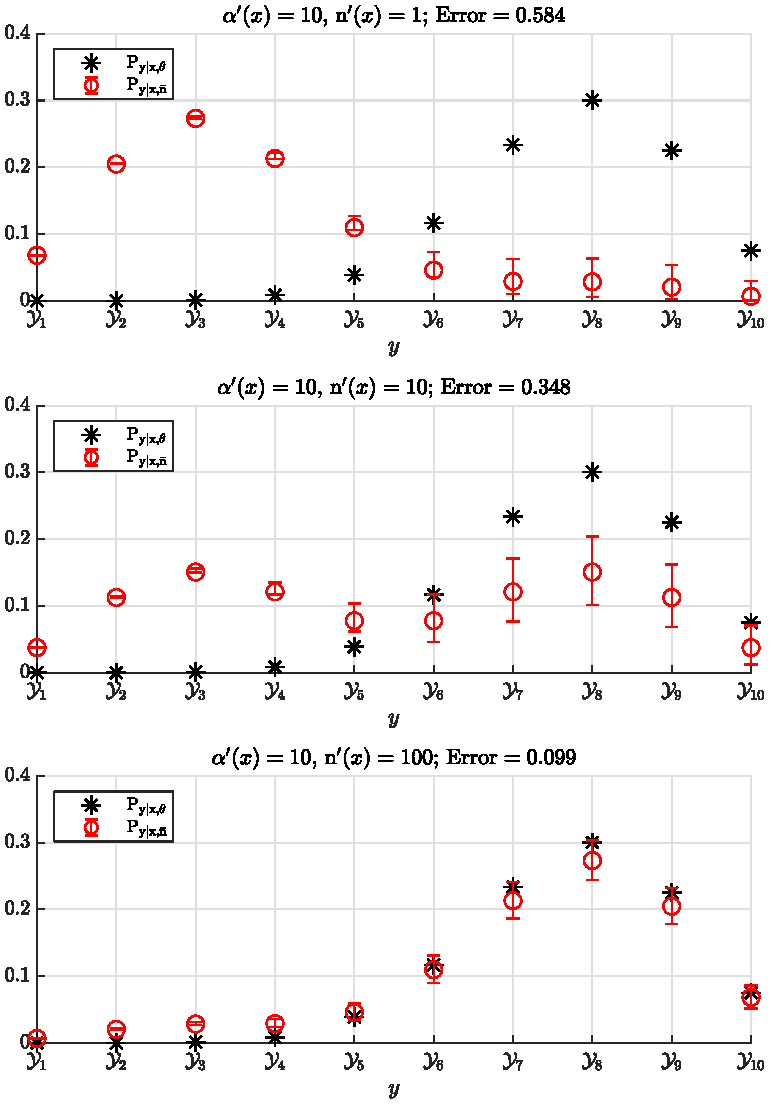
\includegraphics[width=1\linewidth]{P_yx_error_a0_10.pdf}
%\caption{Model $\uptheta$ estimates, $\alpha_0 = 10$}
%\label{fig:P_yx_error_a0_10}
\end{figure}
\end{column}

\end{columns}

\end{frame}




\begin{frame}
\frametitle{Application to Common Loss Functions}
\framesubtitle{Regularized Empirical Risk}

\begin{itemize}
\item Recall that the Bayesian decision is $f^*(\xrm;\nbarrm) = \argmin_{h \in \Hcal} \Erm_{\yrm | \xrm,\nbarrm} \big[ \Lcal(h,\yrm) \big]$. The Bayesian conditional risk objective for a Dirichlet prior is:
\begin{IEEEeqnarray*}{L} \label{eq:E_y|xD L}
\Erm_{\yrm | \xrm,\nbarrm} \big[ \Lcal(h,\yrm) \big] \\
\equiv \left(\frac{\alpha'(\xrm)}{\alpha'(\xrm) + \nrm'(\xrm)}\right) \sum_{y \in \Ycal} \frac{\alpha(y,\xrm)}{\alpha'(\xrm)} \Lcal(h,y) + \left(\frac{\nrm'(\xrm)}{\alpha'(\xrm) + \nrm'(\xrm)}\right) \sum_{y \in \Ycal} \frac{\nbarrm(y,\xrm)}{\nrm'(\xrm)} \Lcal(h,y) \\
\end{IEEEeqnarray*}
\vspace{-3em}
\Large
\begin{equation*} 
\Downarrow \quad \Downarrow
\end{equation*}
\normalsize

\item \emph{Convex combination} of the expected risk with respect to two distributions: the prior conditional mean and the conditional empirical distribution. Prior parameters provide a \alert{regularizing term} for the empirical loss
\vspace{0.5em}
\item Relative weight $\alpha'(x) / n'(x)$ for regularizing term tends to zero with training data volume, dictating \alert{empirical risk minimization}

\end{itemize}

\end{frame}



%\begin{frame}
%\frametitle{Regression: the Squared-Error Loss}
%\framesubtitle{Part I: Bayes Estimate}
%
%\begin{itemize}
%\item Setting $\Hcal = \Rbb \supset \Ycal$, the optimal \alert{Bayes estimate} is a convex combination of two mean values:
%
%\begin{IEEEeqnarray*}{rCl} \label{eq:f_opt_SE_dir}
%f^*(\xrm;\nbarrm) & = & \mu_{\yrm | \xrm,\nbarrm} = \left( \frac{\alpha'(\xrm)}{\alpha'(\xrm) + \nrm'(\xrm)} \right) \sum_{y \in \Ycal} y \frac{\alpha(y,\xrm)}{\alpha'(\xrm)} + \left( \frac{\nrm'(\xrm)}{\alpha'(\xrm) + \nrm'(\xrm)} \right) \sum_{y \in \Ycal} y \frac{\nbarrm(y,\xrm)}{\nrm'(\xrm)}
%\end{IEEEeqnarray*}
%
%\vspace{1em}
%\item \textbf{Minimum Bayes squared-error}: the expected Bayesian predictive variance
%\begin{IEEEeqnarray*}{L}
%\Rcal^* = \Erm_{\xrm,\nbarrm} \left[ \Sigma_{\yrm | \xrm,\nbarrm} \right] = \Erm_{\xrm} \left[ \frac{\Prm_{\xrm}(\xrm) + (\alpha_0+N)^{-1}}{\Prm_{\xrm}(\xrm) + \alpha_0^{-1}} \Sigma_{\yrm | \xrm} \right] 
%\end{IEEEeqnarray*}
%
%\vspace{1em}
%\textit{Note}: $\Prm_{\xrm} \equiv \alpha' / \alpha_0$ and $\Prm_{\yrm | \xrm} \equiv \alpha(\cdot,\xrm) / \alpha'(\xrm)$
%
%\end{itemize}
%
%\end{frame}


\begin{frame}
\frametitle{Regression: the Squared-Error Loss}
\framesubtitle{Part I: Bayes Estimate}


\textbf{Optimal Estimate}: the \emph{Bayes predictive mean} ($\Hcal = \Rbb \supset \Ycal$)
\vspace{0.25em}
\begin{IEEEeqnarray*}{rCl} \label{eq:f_opt_SE_dir}
f^*(\xrm;\nbarrm) & = & \mu_{\yrm | \xrm,\nbarrm} = \left( \frac{\alpha'(\xrm)}{\alpha'(\xrm) + \nrm'(\xrm)} \right) \sum_{y \in \Ycal} y \frac{\alpha(y,\xrm)}{\alpha'(\xrm)} + \left( \frac{\nrm'(\xrm)}{\alpha'(\xrm) + \nrm'(\xrm)} \right) \sum_{y \in \Ycal} y \frac{\nbarrm(y,\xrm)}{\nrm'(\xrm)}
\end{IEEEeqnarray*}
%
\begin{itemize}
\item[$*$] Convex combination of \alert{prior estimate} $\mu_{\yrm | \xrm} \equiv \sum_{y \in \Ycal} y \frac{\alpha(y,\xrm)}{\alpha'(\xrm)}$ and \alert{empirical mean}
\end{itemize}

\hrulefill
\vspace{1em}

\textbf{Minimum Bayes Squared-Error}: the expected Bayesian predictive variance
\vspace{0.25em}
\begin{IEEEeqnarray*}{L}
\Rcal^* = \Erm_{\xrm,\nbarrm} \left[ \Sigma_{\yrm | \xrm,\nbarrm} \right] = \Erm_{\xrm} \left[ \frac{\Prm_{\xrm}(\xrm) + (\alpha_0+N)^{-1}}{\Prm_{\xrm}(\xrm) + \alpha_0^{-1}} \Sigma_{\yrm | \xrm} \right] 
\end{IEEEeqnarray*}
\vspace{-0.25em}
\begin{itemize}
\item[$*$] \textit{Note}: $\Prm_{\xrm} \equiv \alpha' / \alpha_0$ and $\Prm_{\yrm | \xrm} \equiv \alpha(\cdot,\xrm) / \alpha'(\xrm)$
\end{itemize}




\end{frame}



\begin{frame}
\frametitle{Regression: the Squared-Error Loss}
\framesubtitle{Part II: Minimum Bayes Risk Trends}

\begin{itemize}
\item Unit interval:  $\Ycal = \{ i/M_{\yrm} : i = 0,\ldots,M_{\yrm}-1 \}$, $\Xcal = \{ i/M_{\xrm} : i = 0,\ldots,M_{\xrm}-1 \}$
\end{itemize}

\begin{columns}[c]

\begin{column}{0.5\linewidth}
\begin{figure}
\centering
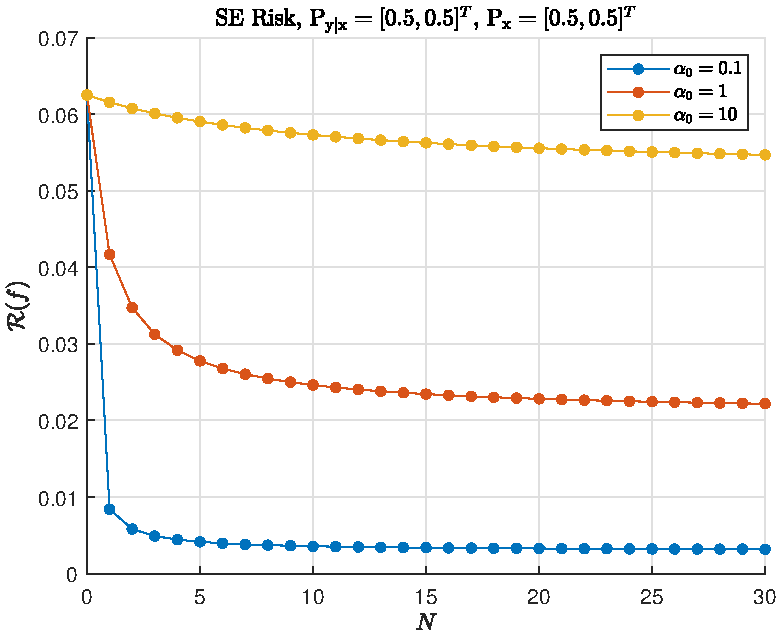
\includegraphics[width=0.9\linewidth]{Risk_SE_Dir_IO_N_leg_a0.pdf}
%\caption{Minimum SE Risk for different training set sizes $N$}
%\label{fig:Risk_SE_Dir_IO_N_leg_a0}
\end{figure}
%
\vspace{-0.25em}
\begin{equation*}
\lim_{N \to \infty} \Rcal^* \equiv \Erm_{\xrm} \left[ \frac{\Prm_{\xrm}(\xrm)}{\Prm_{\xrm}(\xrm) + \alpha_0^{-1}} \Sigma_{\yrm | \xrm} \right] 
\end{equation*}

\end{column}

\begin{column}{0.5\linewidth}
\begin{figure}
\centering
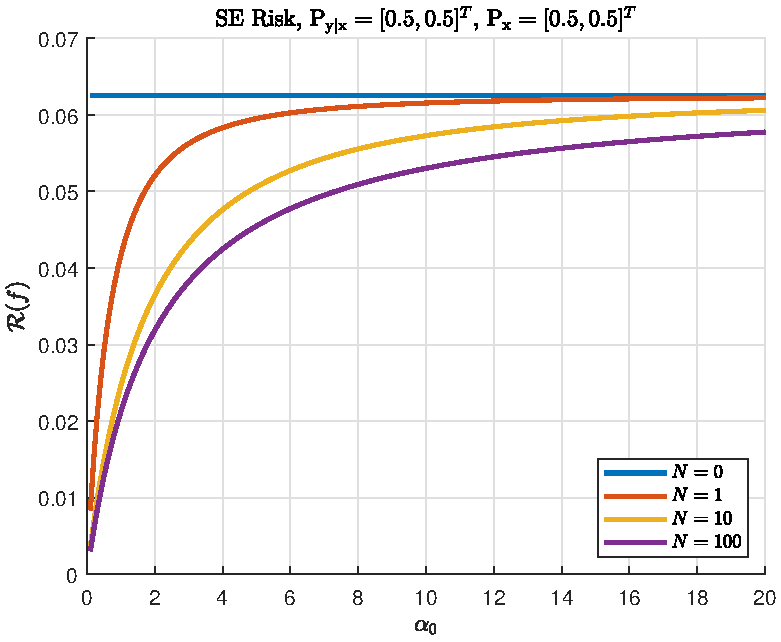
\includegraphics[width=0.9\linewidth]{Risk_SE_Dir_IO_a0_leg_N.pdf}
%\caption{Minimum SE Risk for different prior concentrations $\alpha_0$}
%\label{fig:Risk_SE_Dir_IO_a0_leg_N}
\end{figure}
%
\vspace{-0.25em}
\begin{equation*}
\lim_{\alpha_0 \to \infty} \Rcal^* \equiv \Erm_{\xrm} \left[ \Sigma_{\yrm | \xrm} \right]
\end{equation*}

\end{column}

\end{columns}

\end{frame}




\begin{frame}
\frametitle{Regression: the Squared-Error Loss}
\framesubtitle{Part III: Conditional Risk}

General squared-error $\Rcal_{\Theta}(f ; \uptheta)$ is the sum of the clairvoyant risk $\Rcal_{\Theta}^*(\uptheta) = \Erm_{\xrm | \uptheta} \left[ \Sigma_{\yrm | \xrm,\uptheta} \right]$ and the \alert{expected squared-bias} between the clairvoyant estimate $f_{\Theta}(\xrm;\uptheta) = \mu_{\yrm | \xrm,\uptheta}$ and the Bayes estimate $\mu_{\yrm | \xrm,\nbarrm}$
%
\vspace{0.5em}
\begin{IEEEeqnarray*}{rCl} \label{eq:risk_cond_SE_dir_ex}
\Rcal_{\Theta, \mathrm{ex}}(f^* ; \uptheta) & = & \Erm_{\xrm,\nbarrm | \uptheta} \Big[ \big( \mu_{\yrm | \xrm,\nbarrm} - \mu_{\yrm | \xrm,\uptheta} \big)^2 \Big] \\
& = & \Erm_{\xrm | \uptheta}\left[ \alert{\Sigma_{\yrm | \xrm,\uptheta}} \Erm_{\nrm'(\xrm) | \uptheta'(\xrm)}\left[ \frac{\nrm'(\xrm)}{\big( \alpha'(\xrm) + \nrm'(\xrm) \big)^2} \right] \right] \\
&& \qquad + \Erm_{\xrm | \uptheta}\left[ \alert{\left( \mu_{\yrm | \xrm} - \mu_{\yrm | \xrm,\uptheta} \right)^2} \Erm_{\nrm'(\xrm) | \uptheta'(\xrm)}\left[ \left(\frac{\alpha'(\xrm)}{\alpha'(\xrm) + \nrm'(\xrm)}\right)^2 \right] \right] 
\end{IEEEeqnarray*}

\vspace{0.25em}
\footnotesize
\textit{Note}: Scaling via expectations of $\nrm'(x) | \uptheta'(x) \sim \Bi \big(N,\uptheta'(x)\big)$
\normalsize

\vspace{0.5em}
\centering
\fcolorbox{bumper}{bumper}{\color{white}
\parbox{36em}{
\centering
\large
\textbf{Excess squared-error combines an excess variance term and \\a squared-bias term for the data-independent estimate $\bm{\mu_{\yrm | \xrm}}$}
}
}

\end{frame}





\begin{frame}
\frametitle{Regression: the Squared-Error Loss}
\framesubtitle{Part IV: Conditional Risk Trends}

\begin{columns}[c]

\begin{column}{0.5\linewidth}

\centering
\textbf{Unbiased}: $\mu_{\yrm | \xrm} - \mu_{\yrm | \xrm,\uptheta} = 0$
%
\begin{figure}
\centering
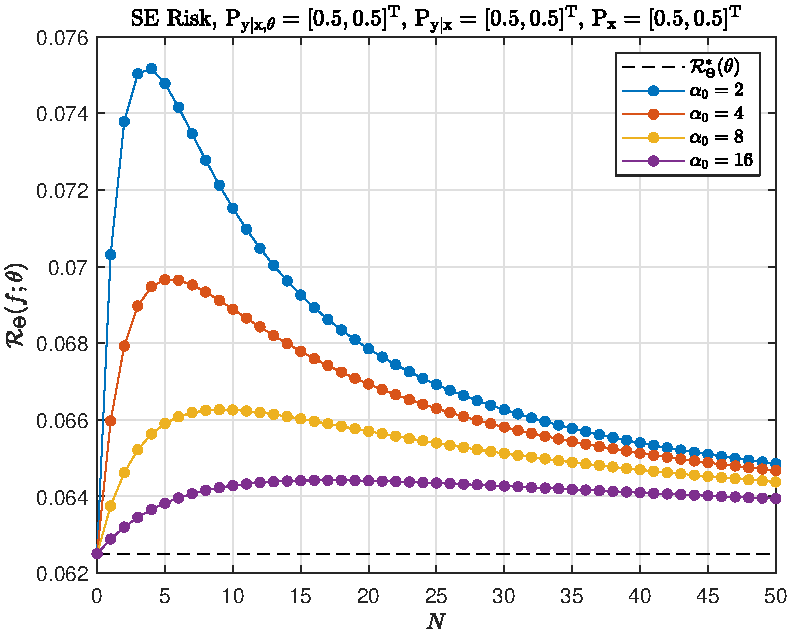
\includegraphics[width=1\linewidth]{Risk_cond_SE_Dir_N_leg_a0_unbiased.pdf}
%\caption{Conditional SE Risk versus $N$, unbiased Dirichlet estimators of varying concentration}
%\label{fig:Risk_cond_SE_Dir_N_leg_a0_unbiased}
\end{figure}


\end{column}

\begin{column}{0.5\linewidth}

\centering
\textbf{Biased}: $\mu_{\yrm | \xrm} - \mu_{\yrm | \xrm,\uptheta} \neq 0$
%
\begin{figure}
\centering
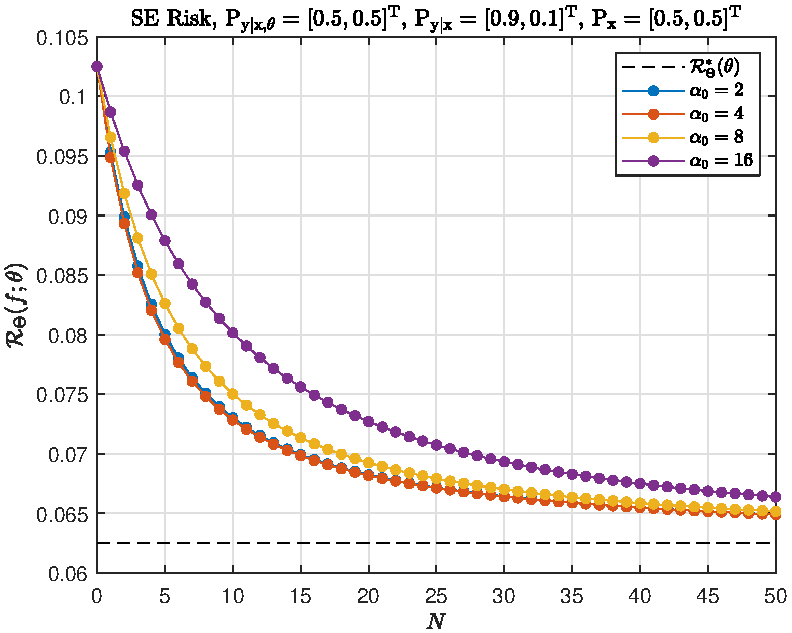
\includegraphics[width=1\linewidth]{Risk_cond_SE_Dir_N_leg_a0_biased.pdf}
%\caption{Conditional SE Risk versus $N$, biased Dirichlet estimators of varying concentration}
%\label{fig:Risk_cond_SE_Dir_N_leg_a0_biased}
\end{figure}

\end{column}

\end{columns}

\centering
\fcolorbox{bumper}{bumper}{\color{white}
\parbox{36em}{
\centering
\large
\textbf{Full prior support guarantees $\bm{\mathcal{R}_{\Theta, \mathrm{ex}}(f^* ; \uptheta) \to 0}$ as $\bm{N \to \infty}$}
}
}

\end{frame}




\begin{frame}
\frametitle{Regression: the Squared-Error Loss}
\framesubtitle{Part IV: Conditional Risk Trends}

\textbf{Conditional concentration $\alpha'(x)$ controls the Bias-Variance risk trade-off}


\begin{columns}[c]

\begin{column}{0.55\linewidth}



\begin{block}{Excess Risk $\Rcal_{\Theta, \mathrm{ex}}(f^* ; \uptheta)$}

\small
\vspace{1em}
\underline{$\alpha'(x) \to 0$}:
\vspace{0.25em}

$\approx \Erm_{\xrm | \uptheta}\left[ \Sigma_{\yrm | \xrm,\uptheta} \sum_{n=1}^N \binom{N}{n} \uptheta'(\xrm)^n \big( 1 - \uptheta'(\xrm) \big)^{N-n} \frac{1}{n} \right] $

\vspace{2.25em}
\underline{$\alpha'(x) \to \infty$}:
\vspace{0.25em}

$= \Erm_{\xrm | \uptheta}\left[ \left( \mu_{\yrm | \xrm} - \mu_{\yrm | \xrm,\uptheta} \right)^2 \right]$

\end{block}

%\begin{IEEEeqnarray*}{L}
%\lim_{\alpha'(x) \to 0} \Rcal_{\Theta, \mathrm{ex}}(f^* ; \uptheta) \\
% \approx \Erm_{\xrm | \uptheta}\left[ \Sigma_{\yrm | \xrm,\uptheta} \sum_{n=1}^N \binom{N}{n} \uptheta'(\xrm)^n \big( 1 - \uptheta'(\xrm) \big)^{N-n} \frac{1}{n} \right] 
%\end{IEEEeqnarray*}
%\vspace{2em}
%\begin{IEEEeqnarray*}{L}
%\lim_{\alpha'(x) \to \infty} \Rcal_{\Theta, \mathrm{ex}}(f^* ; \uptheta) 
%= \Erm_{\xrm | \uptheta}\left[ \left( \mu_{\yrm | \xrm} - \mu_{\yrm | \xrm,\uptheta} \right)^2 \right]
%\end{IEEEeqnarray*}

\normalsize

\end{column}

\begin{column}{0.45\linewidth}

\begin{figure}
\centering
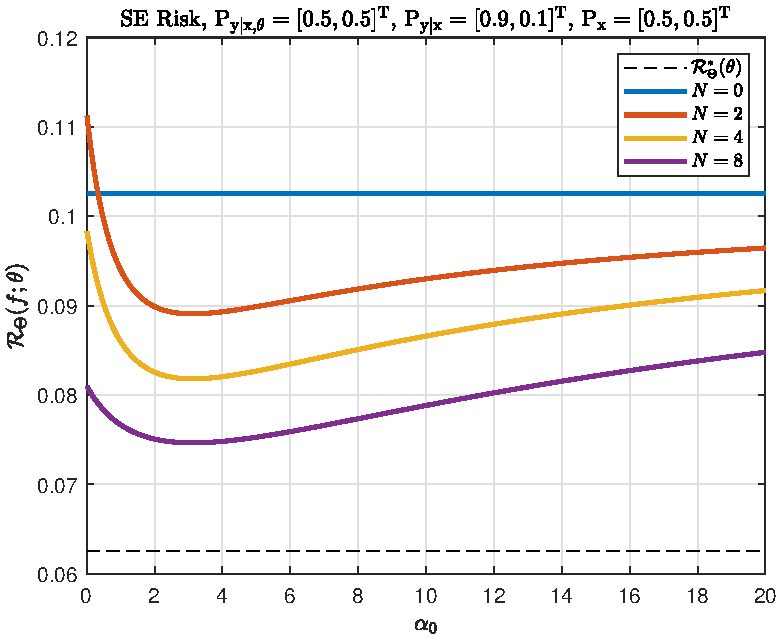
\includegraphics[width=1\linewidth]{Risk_cond_SE_Dir_a0_leg_N_biased.pdf}
%\caption{Conditional SE Risk versus $\alpha'(x)$, biased Dirichlet estimator using varying training set volumes}
%\label{fig:Risk_cond_SE_Dir_a0_leg_N_biased}
\end{figure}

\end{column}

\end{columns}

\centering
\fcolorbox{bumper}{bumper}{\color{white}
\parbox{37em}{
\centering
\large
\textbf{Concentration $\bm{\alpha'(x) \equiv \frac{\Sigma_{\yrm | \xrm,\uptheta} }{ \left( \mu_{\yrm | \xrm} - \mu_{\yrm | \xrm,\uptheta} \right)^2}}$ minimizes squared-error given $\bm{\mathrm{P}_{\yrm | \xrm}}$}
}
}

\end{frame}




%\begin{frame}
%\frametitle{Classification: the 0--1 Loss}
%\framesubtitle{Part I}
%
%\textbf{Optimal Hypothesis}: \emph{weighted conditional majority decision}
%\begin{IEEEeqnarray*}{rCl} \label{eq:f_opt_01_dir}
%f^*(x;\bar{n}) & = & \argmax_{y \in \Ycal} \Prm_{\yrm | \xrm,\nbarrm}(y | x,\bar{n}) = \argmax_{y \in \Ycal} \left( \alpha(y,x) + \bar{n}(y,x) \right)
%\end{IEEEeqnarray*}
%
%\hrulefill
%\vspace{0.5em}
%
%\textbf{Minimum Bayes Probability of Error}:
%\begin{IEEEeqnarray*}{rCl}
%\Rcal^* & = & 1 - \Erm_{\xrm,\nbarrm} \left[ \max_{y \in \Ycal} \Prm_{\yrm | \xrm,\nbarrm}(y | \xrm,\nbarrm) \right] = 1 - \sum_{x \in \Xcal} \frac{\Erm_{\nbarrm} \Big[ \max_{y \in \Ycal} \big( \alpha(y,x) + \bar{\nrm}(y,x) \big) \Big]}{\alpha_0 + N} 
%\end{IEEEeqnarray*}
%\vspace{0.5em}
%
%
%\end{frame}

\begin{frame}
\frametitle{Classification: the 0--1 Loss}
\framesubtitle{Part I: Bayes Classifier}

\begin{columns}[c]

\begin{column}{.5\linewidth}

\textbf{Optimal Hypothesis}: 

\emph{Weighted conditional majority decision}
\begin{IEEEeqnarray*}{rCl} \label{eq:f_opt_01_dir}
f^*(x;\bar{n}) & = & \argmax_{y \in \Ycal} \Prm_{\yrm | \xrm,\nbarrm}(y | x,\bar{n}) \\
& = & \argmax_{y \in \Ycal} \left( \alpha(y,x) + \bar{n}(y,x) \right)
\end{IEEEeqnarray*}

\hrulefill
\vspace{0.5em}

\textbf{Minimum Bayes Probability of Error}:
\begin{IEEEeqnarray*}{rCl}
\Rcal^* & = & 1 - \Erm_{\xrm,\nbarrm} \left[ \max_{y \in \Ycal} \Prm_{\yrm | \xrm,\nbarrm}(y | \xrm,\nbarrm) \right] \\
& = & 1 - \sum_{x \in \Xcal} \frac{\Erm_{\nbarrm} \Big[ \max_{y \in \Ycal} \big( \alpha(y,x) + \bar{\nrm}(y,x) \big) \Big]}{\alpha_0 + N} 
\end{IEEEeqnarray*}
\vspace{0.5em}

\end{column}

\hspace{1ex}
\begin{column}{.5\linewidth}

\begin{figure}
\centering
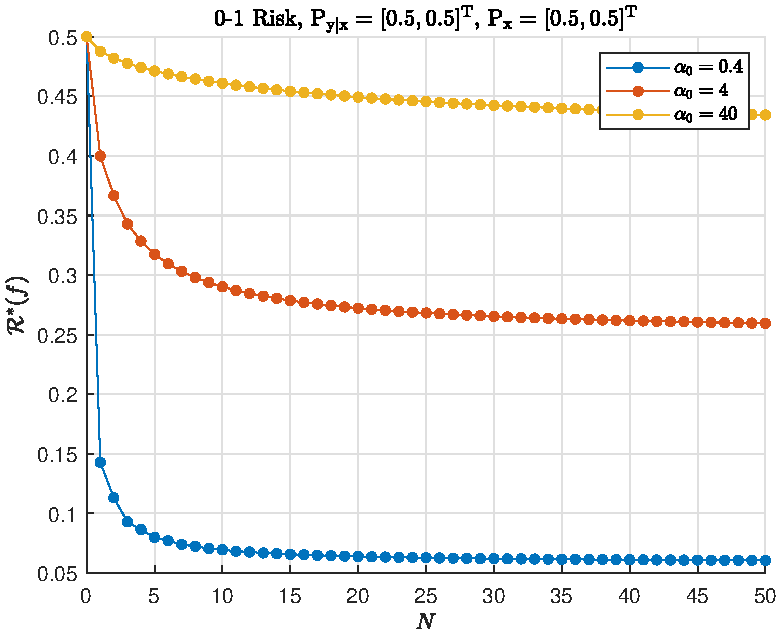
\includegraphics[width=1\linewidth]{Risk_01_Dir_N_leg_a0.pdf}
%\caption{Minimum 0-1 Risk for different training data volumes $N$}
%\label{fig:Risk_01_Dir_N_leg_a0}
\end{figure}

\end{column}


\end{columns}


\end{frame}



\begin{frame}
\frametitle{Classification: the 0--1 Loss}
\framesubtitle{Part II: Conditional Majority Decision}



\begin{columns}[c]

\begin{column}{.55\linewidth}

%With \alert{minimally localized} ($\alpha_0 \to 0$) or \alert{non-informative} ($\alpha = 1$) priors, the majority decision minimizes the empirical risk
With a \alert{non-informative} ($\alpha = 1$) prior, the majority decision minimizes the empirical risk
\begin{IEEEeqnarray}{rCl} 
f^*(x;\bar{n}) & = & \argmax_{y \in \Ycal} \bar{n}(y,x) \nonumber
\end{IEEEeqnarray}
%
\footnotesize
\begin{IEEEeqnarray*}{L}
\Rcal^* = 1 - \frac{\sum_{m=1}^{|\Ycal|} \binom{|\Ycal|}{m} (-1)^{m-1} \sum_{n=0}^{\big\lfloor\frac{N}{m}\big\rfloor} \prod_{l=1}^{|\Ycal||\Xcal|-1} \Big( 1-\frac{mn}{N+l} \Big)}{|\Ycal| + N/|\Xcal|} 
\end{IEEEeqnarray*}
\normalsize

\end{column}

\hspace{3ex}
\begin{column}{.45\linewidth}

\begin{figure}
\centering
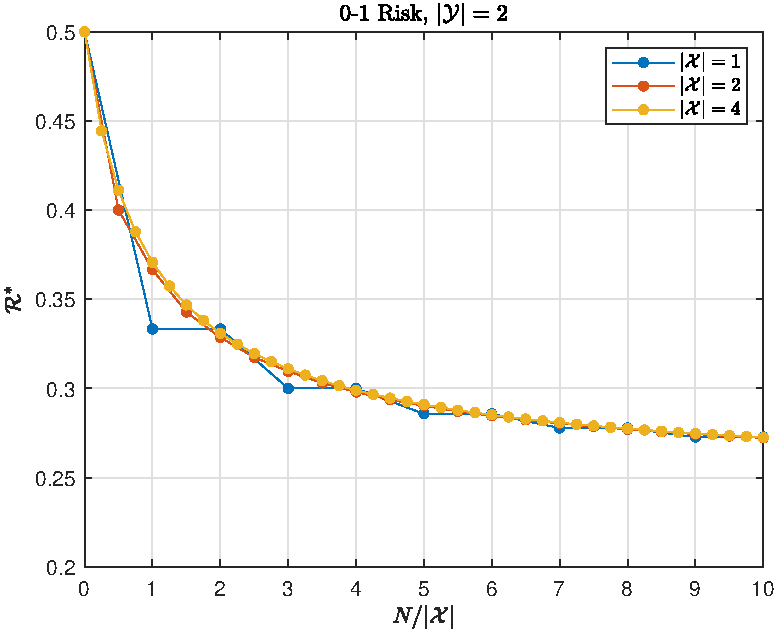
\includegraphics[width=0.9\linewidth]{Risk_01_uni_N-Mx.pdf}
%\caption{Minimum 0-1 Risk vs $N/|\Xcal|$}
%\label{fig:Risk_01_uni_N-Mx}
\end{figure}

\end{column}

\end{columns}

\vspace{1em}
\begin{itemize}
\item \alert{Computationally efficient} formula derived using \emph{Inclusion-Exclusion principle}
\vspace{0.25em}
\item Minimal risk can be approximated by a function dependent only on $N/|\Xcal|$
\end{itemize}

\end{frame}



\begin{frame}
\frametitle{Classification: the 0--1 Loss}
\framesubtitle{Part II: Conditional Majority Decision}

\begin{columns}[c]

\begin{column}{.5\linewidth}

\begin{itemize}
\item For binary classification, infinite training data reduces the expected probability of error only from \alert{0.5} to \alert{0.25}
\vspace{0.5em}
\item As $|\Ycal|$ increases, the probability of error tends to unity and any improvement due to training data becomes \alert{negligible}
\end{itemize}

\begin{table}
\renewcommand{\arraystretch}{1.3}
\begin{tabular}{| c | c |}
\hline 
$N$ & $\Rcal^*$ \\
\hhline{|=|=|}
$0$ & $1 - |\Ycal|^{-1}$  \\ 
\hline
$\to \infty$ & $1 - |\Ycal|^{-1} \sum_{m=1}^{|\Ycal|} m^{-1}$ \\
\hline
\end{tabular}
%\caption{}
\end{table}

\end{column}

\begin{column}{.5\linewidth}

\begin{figure}
\centering
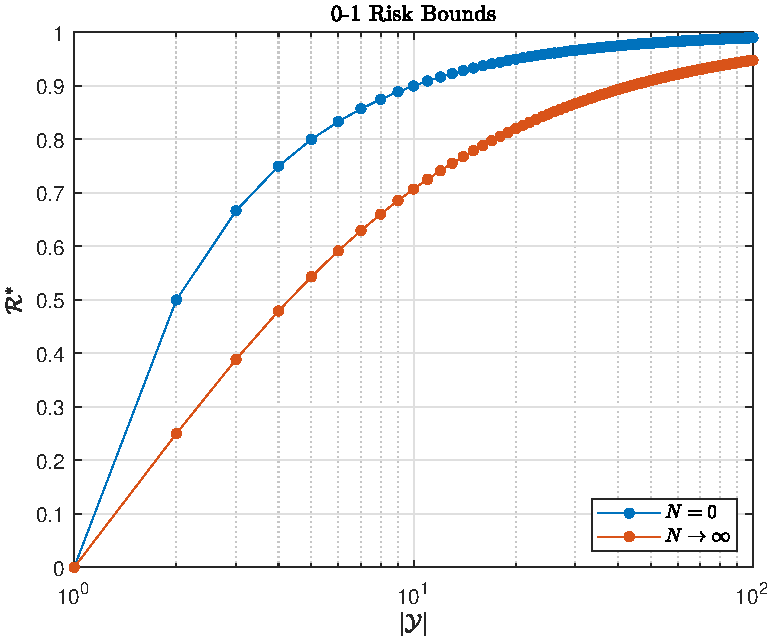
\includegraphics[width=1\linewidth]{Risk_01_uni_N_bounds.pdf}
%\caption{Minimum 0--1 Risk for zero and infinite number of training data}
\label{fig:Risk_01_uni_N_bounds}
\end{figure}

\end{column}

\end{columns}

\end{frame}




\begin{frame}
\frametitle{Classification: the 0--1 Loss}
\framesubtitle{Part III: Conditional Risk Trends}

\begin{columns}[c]

\begin{column}{0.5\linewidth}

\centering
\textbf{Accurate Prior}: $\argmax_{y \in \Ycal} \alpha(y,x) = \argmax_{y \in \Ycal} \tilde{\theta}(y;x)$
%
\begin{figure}
\centering
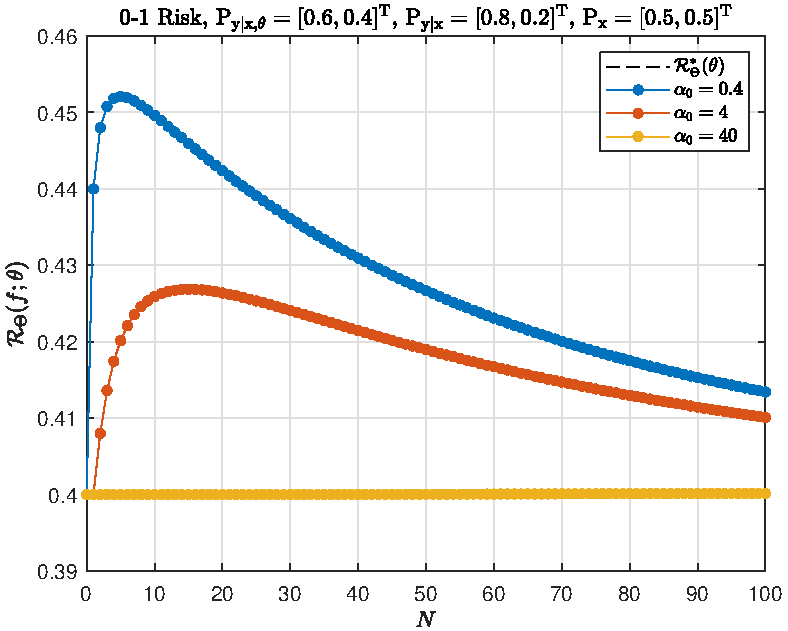
\includegraphics[width=0.9\linewidth]{Risk_cond_01_Dir_N_leg_a0__subj_good.pdf}
%\caption{Excess conditional probability of error, well-matched informative Dirichlet-based classifier}
%\label{fig:Risk_cond_01_Dir_N_leg_a0__subj_good}
\end{figure}


\end{column}

\begin{column}{0.5\linewidth}

\centering
\textbf{Inaccurate Prior}: $\argmax_{y \in \Ycal} \alpha(y,x) \neq \argmax_{y \in \Ycal} \tilde{\theta}(y;x)$
%
\begin{figure}
\centering
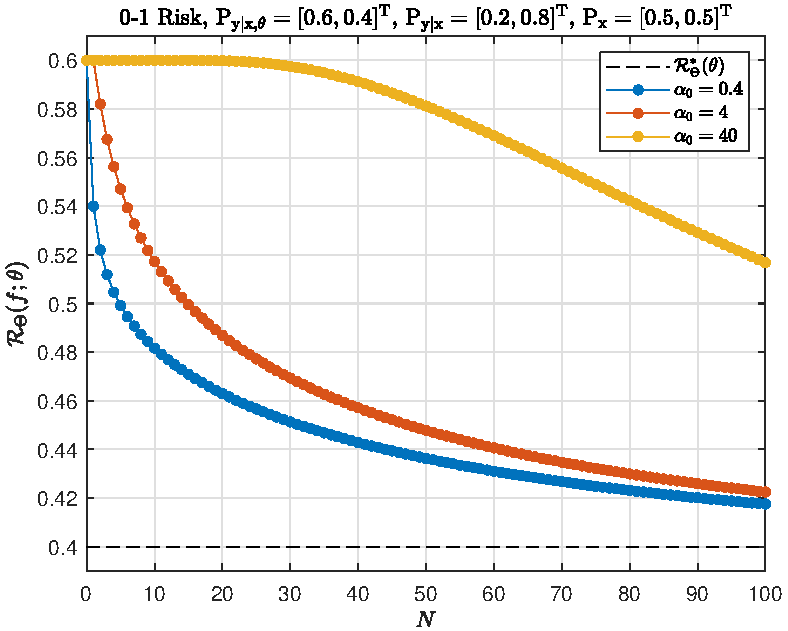
\includegraphics[width=0.9\linewidth]{Risk_cond_01_Dir_N_leg_a0__subj_bad.pdf}
%\caption{Excess conditional probability of error, poorly-matched informative Dirichlet-based classifier}
%\label{fig:Risk_cond_01_Dir_N_leg_a0__subj_bad}
\end{figure}

\end{column}

\end{columns}

\centering
\fcolorbox{bumper}{bumper}{\color{white}
\parbox{36em}{
\centering
\large
\textbf{Full prior support guarantees $\bm{\mathcal{R}_{\Theta, \mathrm{ex}}(f^* ; \uptheta) \to 0}$ as $\bm{N \to \infty}$}
}
}

\end{frame}




\begin{frame}
\frametitle{Classification: the 0--1 Loss}
\framesubtitle{Part III: Conditional Risk Trends}

%\vspace{-1em}
\begin{columns}[c]

\begin{column}{.5\linewidth}

\centering
\textbf{Non-informative Prior}:
%
\begin{figure}
\centering
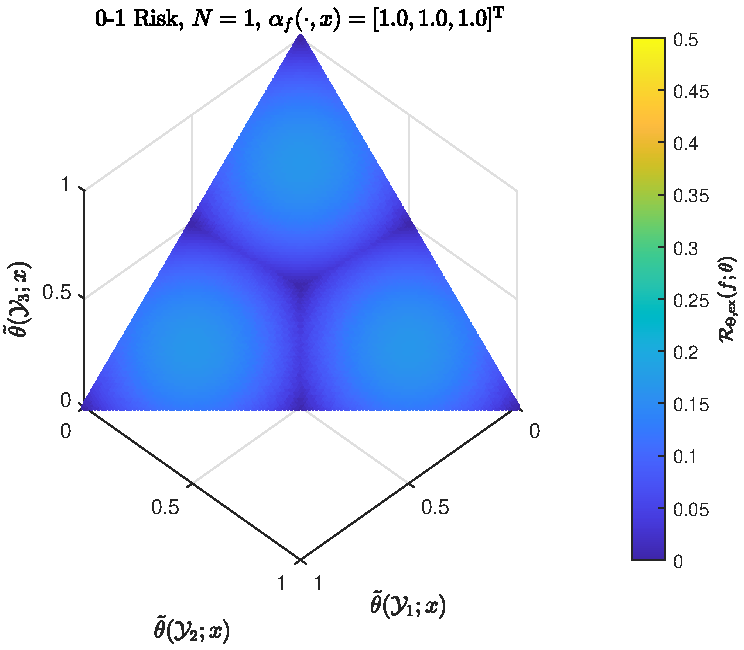
\includegraphics[width=0.8\linewidth]{Risk_cond_ex_01_Dir_theta__uni_clim.pdf}
%\caption{}
\label{fig:Risk_cond_ex_01_Dir_theta__uni}
\end{figure}

\end{column}

\begin{column}{.5\linewidth}

\centering
\textbf{Informative Prior}:
%
\begin{figure}
\centering
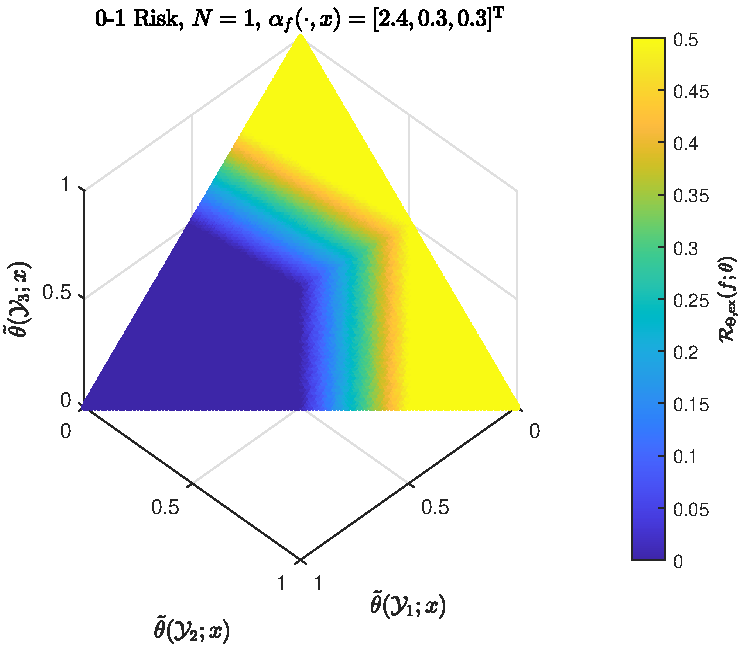
\includegraphics[width=0.8\linewidth]{Risk_cond_ex_01_Dir_theta__subj_clim.pdf}
%\caption{}
\label{fig:Risk_cond_ex_01_Dir_theta__subj}
\end{figure}

\end{column}

\end{columns}

%\vspace{-0.2em}
\begin{block}{Trade-Off}
\textbf{Uniform prior provides a robust classifier for all unknown models $\theta$, limiting the space of high-error models. However, fewer models achieve the clairvoyant risk}
\end{block}


\end{frame}






\section{Plan for Completion}


\begin{frame}
\frametitle{Learning with Low-Dimensionality Support Priors}

\begin{itemize}
\item Additional theory needs to be developed for Bayesian learning using priors with limited dimensionality support
\vspace{0.25em}
	\vspace{0.25em}
	\begin{itemize}
	\item Quantify risk $\Rcal_{\Theta}(f ; \uptheta)$ for \alert{limited volume $N$}, compare to full-support and non-informative prior results
	\vspace{0.25em}
	\item Assess additional risk beyond clairvoyant $\Rcal_{\Theta}^*(\uptheta)$ incurred in the limit $N \to \infty$
	\vspace{0.25em}
	\item Determine relationship between $\dim(\Theta) < |\Ycal||\Xcal| - 1$ and \alert{computational complexity} of implementation. Can data be sufficiently represented after mapping to a set with cardinality $< |\bar{\Ncal}|$?
%	Simpler optimal data representation, $|\Dcal| \Rightarrow |\bar{\Ncal}| \Rightarrow \bm{???}$
	\end{itemize}
\vspace{0.5em}
\item Specific research for class of mixture distributions $\uptheta \equiv \sum_{m = 1}^M \upphi_m h_m$, where $h_m \in \Theta$
	\vspace{0.25em}
	\begin{itemize}
	\item Hyperparameters $\phi$ are convex coefficients $\Rightarrow$ characterize with Dirichlet distribution
	\vspace{0.25em}
	\item If mixture distributions have disjoint support $h_i(y,x) \cdot h_j(y,x) = 0$, likelihood $\Prm_{\Drm | \upphi}$ has \alert{exponential form}
	\end{itemize}

\end{itemize}

\end{frame}



\begin{frame}
\frametitle{Apply to Human Recognition Tasks}

\begin{itemize}
\item Bayesian learners will be applied first to \alert{simulated data} $\xrm \in \Xcal = \{0,1\}^K$ and subsequently to more complex recognition \alert{benchmark data}
\vspace{0.5em}
\item Simulated data below (random translations/rotations) demonstrates properties that motivate the use of \alert{low-dimensionality support} priors
	\vspace{0.25em}
	\begin{itemize}
	\item Only $9+2(9) = 27$ images $x$ are ever observed, compared to the $2^{25} = 33554432$ possible binary images $\Rightarrow$ Prior should be restricted by $\big\| \theta' \big\|_0 \ll |\Xcal|$ 
	\vspace{0.25em}
	\item Each data sample $x$ is unique to a single class, such that $\big\| \tilde{\theta}(x) \big\|_{\infty} = 1$
	\end{itemize}
\end{itemize}


\begin{columns}[c]
\hspace{2ex}
\begin{column}{.4\linewidth}
\begin{figure}
\centering
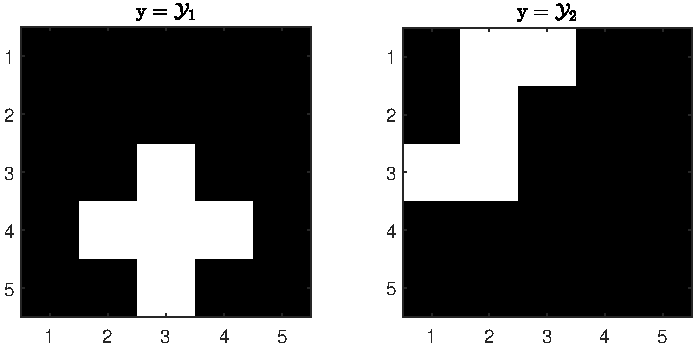
\includegraphics[width=1\linewidth]{character_sim_ex.pdf}
%\caption{Simulated character recognition data}
%\label{fig:character_sim_ex}
\end{figure}
\end{column}

\begin{column}{0.03\linewidth}
\Huge
$\Rightarrow$
\normalsize
\end{column}

\begin{column}{.25\linewidth}
\begin{figure}
\centering
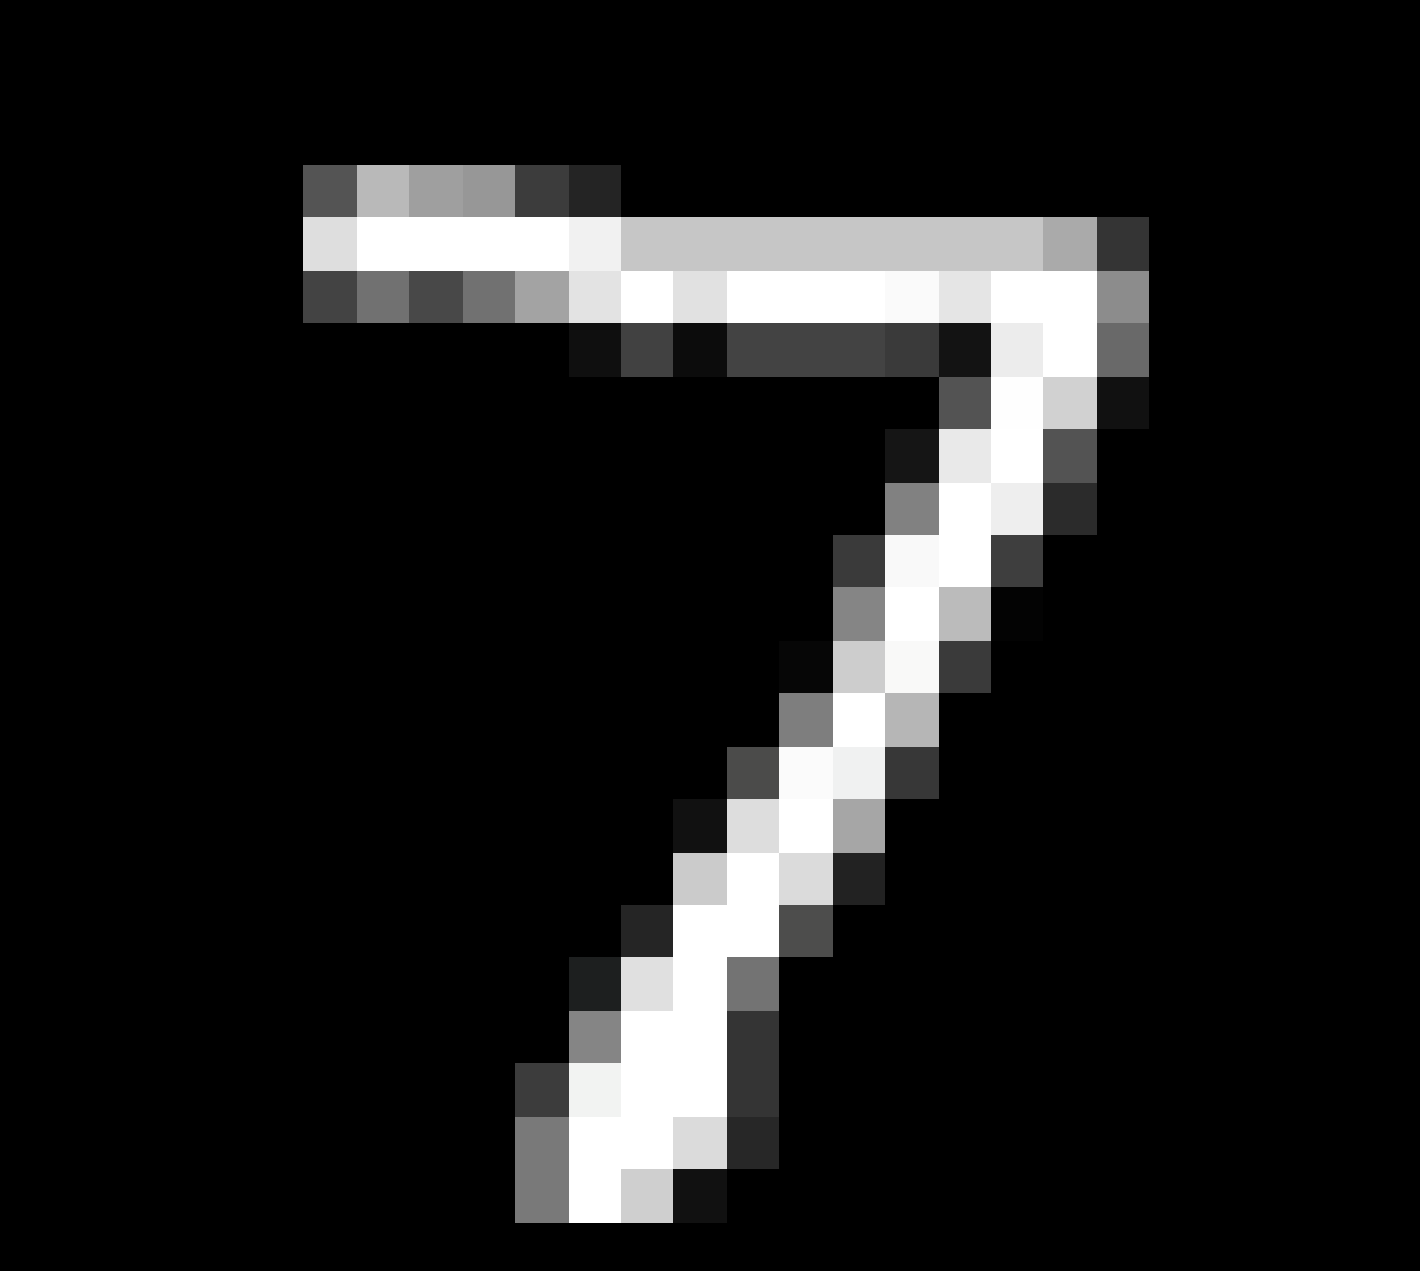
\includegraphics[width=0.8\linewidth]{mnist_digit_sample.png}
%\caption{}
\end{figure}
\end{column}

\begin{column}{0.03\linewidth}
\Huge
$\Rightarrow$
\normalsize
\end{column}

\begin{column}{.25\linewidth}
\begin{figure}
\centering
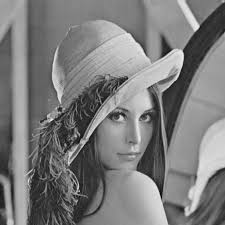
\includegraphics[width=0.8\linewidth]{lena.jpg}
%\caption{}
\end{figure}
\end{column}

\end{columns}


\end{frame}



\begin{frame}
\frametitle{Generalize Theory for Uncountably Infinite Sets}

\begin{itemize}
\item Initial work assumes finite sets $\Ycal$ and $\Xcal$, since digital machine learning functions unavoidably use finite data representations. However, numerical data with $|\Xcal| \gg 1$ can often be approximated with real numbers, motivating an analysis for \alert{continuous data}
\vspace{0.5em}
\item Extending to Euclidean sets (starting with $\Ycal = \Xcal = \Rbb$), the model $\uptheta$ is treated as a \alert{random process}
	\vspace{0.25em}
	\begin{itemize}
	\item Dirichlet process $\uptheta \sim \DP(\alpha)$ inherits the desirable properties of the PDF \footfullcite{bishop}
	\vspace{0.25em}
	\item Empirical process $\nbarrm \equiv \sum_{n=1}^N \delta\left( \cdot - \Drm_n \right)$ characterized by new concepts: the \alert{Multinomial Process} and the \alert{Dirichlet-Multinomial Process}
	\end{itemize}
\vspace{0.5em}
\item Analysis of learning with limited-dimensionality priors will generalize naturally to continuous data sets
	\vspace{0.25em}
	\begin{itemize}
	\item \emph{Example}: Model $\uptheta$ as a finite mixture of continuous distributions $h_m$
	\end{itemize}
\end{itemize}

\end{frame}



\begin{frame}
\frametitle{Expand Framework for Joint Decisions and Semi-Supervised Learning}

\begin{itemize}
\item With a Dirichlet prior, the model posterior $\prm_{\tilde{\uptheta} | \xrm,\Drm}$ has no dependency on the novel observation $\xrm$; using general priors, the datum $\xrm$ refines our statistical understanding of the model, effecting \alert{semi-supervised} learning 
\vspace{0.5em}
\item Generalization to $L$ joint decisions $(h_1,\ldots,h_L) \in \Hcal^L$ based on observations $(\xrm_1,\ldots,\xrm_L) \in \Xcal^L$, each corresponding to a distinct unobserved random element $(\yrm_1,\ldots,\yrm_L) \in \Ycal^L$
\vspace{0.25em}
	\begin{itemize}
	\item \alert{Sample risk} comparison with popular non-Bayesian learners using training data $\Drm$ and test data $\big( (\yrm_1,\xrm_1),\ldots,(\yrm_L,\xrm_L)\big)$
	\vspace{0.25em}
	\item Dirichlet prior dictates \alert{independent decisions} due to conditional independence of the model $\tilde{\uptheta}$ from the novel observations $(\xrm_1,\ldots,\xrm_L)$
	\end{itemize}
\vspace{0.5em}
\item Semi-supervised risk trends for $L \to \infty$ will be a primary research focus
\end{itemize}

\end{frame}


%\begin{frame}[allowframebreaks]
%\frametitle{References}
%\small
%\setbeamertemplate{bibliography item}[text]
%%\bibliographystyle{amsplain}
%\bibliographystyle{amsalpha}
%%\bibliographystyle{IEEEtran}
%\bibliography{{../References/phd_bib}}
%\end{frame}






\end{document}
